\documentclass[aspectratio=43]{beamer}

% Title --------------------------------------------
\title{\huge Civil wars I}
\author{Francisco Villamil}
\date{War, peace, and political violence\\UC3M, Fall 2023}

%%% NOTE -- CHECK THIS: https://github.com/paulgp/beamer-tips


%%% Building heavily on https://github.com/kylebutts/templates

% xcolor, define them
\usepackage{xcolor}

% TEXT COLORS
\definecolor{red}{HTML}{9a2515}
\definecolor{yellow}{HTML}{EBC944}
\definecolor{asher}{HTML}{555F61}
\definecolor{jet}{HTML}{131516}

% THEME COLORS
\definecolor{accent}{HTML}{107895}
\definecolor{accent2}{HTML}{9a2515}

% Color commands
\newcommand\red[1]{{\color{red}#1}}
\newcommand\yellow[1]{{\color{yellow}#1}}
\newcommand\asher[1]{{\color{asher}#1}}

\newcommand\BGred[1]{{\colorbox{red!80!white}{#1}}}
\newcommand\BGyellow[1]{{\colorbox{yellow!80!white}{#1}}}
\newcommand\BGasher[1]{{\colorbox{asher!80!white}{#1}}}

\renewcommand<>{\BGyellow}[1]{\only#2{\beameroriginal{\BGyellow}}{#1}}

% Appendix numbering
\usepackage{appendixnumberbeamer}

% Beamer Options -------------------------------------

% Background
\setbeamercolor{background canvas}{bg = white}

% Change text margins
\setbeamersize{text margin left = 25pt, text margin right = 15pt}

% \alert
\setbeamercolor{alerted text}{fg = accent2}

% Frame title
\setbeamercolor{frametitle}{bg = white, fg = jet}
\setbeamercolor{framesubtitle}{bg = white, fg = accent}
\setbeamerfont{framesubtitle}{size = \small, shape = \itshape}

% Block
\setbeamercolor{block title}{fg = white, bg = accent2}
\setbeamercolor{block body}{fg = jet, bg = jet!10!white}

% Title page
\setbeamercolor{title}{fg = jet}
\setbeamercolor{subtitle}{fg = accent}

%% Custom \maketitle and \titlepage
\setbeamertemplate{title page}
{
    \begin{centering}
      % \vspace{20mm}
      {\Large \usebeamerfont{title}\usebeamercolor[fg]{title}\inserttitle}\\ \vskip0.25em%
      \ifx\insertsubtitle\@empty%
      \else%
        {\usebeamerfont{subtitle}\usebeamercolor[fg]{subtitle}\insertsubtitle\par}%
      \fi%
      {\vspace{10mm}\insertauthor}\\
      \ifx\insertinstitute\@empty%
      \else%
        {\vspace{5mm}\color{asher}\scriptsize{\insertinstitute}}
      \fi%
      {\color{asher}\small{\insertdate}}\\
    \end{centering}
}

% Table of Contents
\setbeamercolor{section in toc}{fg = accent!70!jet}
\setbeamercolor{subsection in toc}{fg = jet}

% Button
\setbeamercolor{button}{bg = accent}

% Remove navigation symbols
\setbeamertemplate{navigation symbols}{}

% Table and Figure captions
\setbeamercolor{caption}{fg=jet!70!white}
\setbeamercolor{caption name}{fg=jet}
\setbeamerfont{caption name}{shape = \itshape}

% Put slide number / total slides at the bottom right
\makeatother
\makeatletter
\setbeamertemplate{footline} %{\hfill\insertframenumber/\inserttotalframenumber}
{%
  \leavevmode%
  \hbox{
  \begin{beamercolorbox}[wd=\paperwidth,ht=2.5ex,dp=1.125ex,leftskip=.3cm,rightskip=.3cm plus1fil]{footlinecolor}%
    \color{asher}{\hfill\insertframenumber/\inserttotalframenumber}
  \end{beamercolorbox}}%
  \vskip0pt%
}
\makeatother
\makeatletter

% Bullet points

%% Fix left-margins
\settowidth{\leftmargini}{\usebeamertemplate{itemize item}}
\addtolength{\leftmargini}{\labelsep}

%% enumerate item color
\setbeamercolor{enumerate item}{fg = accent}
\setbeamerfont{enumerate item}{size = \small}
\setbeamertemplate{enumerate item}{\insertenumlabel.}

%% itemize
\setbeamercolor{itemize item}{fg = accent!70!white}
\setbeamerfont{itemize item}{size = \small}
\setbeamertemplate{itemize item}[circle]
\setlength{\itemsep}{0pt plus 6pt}

%% right arrow for subitems
\setbeamercolor{itemize subitem}{fg = accent!60!white}
\setbeamerfont{itemize subitem}{size = \small}
\setbeamertemplate{itemize subitem}{$\rightarrow$}

\setbeamertemplate{itemize subsubitem}[square]
\setbeamercolor{itemize subsubitem}{fg = jet}
\setbeamerfont{itemize subsubitem}{size = \small}

% References

%% Bibliography Font, roughly matching aea
\setbeamerfont{bibliography item}{size = \footnotesize}
\setbeamerfont{bibliography entry author}{size = \footnotesize, series = \bfseries}
\setbeamerfont{bibliography entry title}{size = \footnotesize}
\setbeamerfont{bibliography entry location}{size = \footnotesize, shape = \itshape}
\setbeamerfont{bibliography entry note}{size = \footnotesize}

\setbeamercolor{bibliography item}{fg = jet}
\setbeamercolor{bibliography entry author}{fg = accent!60!jet}
\setbeamercolor{bibliography entry title}{fg = jet}
\setbeamercolor{bibliography entry location}{fg = jet}
\setbeamercolor{bibliography entry note}{fg = jet}

%% Remove bibliography symbol in slides
\setbeamertemplate{bibliography item}{}





% Links ----------------------------------------------

\usepackage{hyperref}
\hypersetup{
  colorlinks = true,
  linkcolor = accent,
  filecolor = accent,
  urlcolor = accent,
  citecolor = accent,
}


% Line spacing --------------------------------------
\usepackage{setspace}
\setstretch{1.2}


% \begin{columns} -----------------------------------
\usepackage{multicol}


% % Fonts ---------------------------------------------
% % Beamer Option to use custom fonts
% \usefonttheme{professionalfonts}
%
% % \usepackage[utopia, smallerops, varg]{newtxmath}
% % \usepackage{utopia}
% \usepackage[sfdefault,light]{roboto}
%
% % Small adjustments to text kerning
% \usepackage{microtype}



% Remove annoying over-full box warnings -----------
\vfuzz2pt
\hfuzz2pt


% Table of Contents with Sections
\setbeamerfont{myTOC}{series=\bfseries, size=\Large}
\AtBeginSection[]{
        \frame{
            \frametitle{Roadmap}
            \tableofcontents[current]
        }
    }


% References ----------------------------------------
\usepackage[
    citestyle= authoryear,
    style = authoryear,
    natbib = true,
    backend = biber
]{biblatex}

% Smaller font-size for references
\renewcommand*{\bibfont}{\small}

% Remove "In:"
\renewbibmacro{in:}{}

% Color citations for slides
\newenvironment{citecolor}
    {\footnotesize\begin{color}{accent2}}
    {\end{color}}

\newcommand{\citetcolor}[1]{{\footnotesize\textcolor{asher}{\citet{#1}}}}
\newcommand{\citepcolor}[1]{{\footnotesize\textcolor{asher}{\citep{#1}}}}

% Tables -------------------------------------------
% Tables too big
% \begin{adjustbox}{width = 1.2\textwidth, center}
\usepackage{adjustbox}
\usepackage{array}
\usepackage{threeparttable, booktabs, adjustbox}

% Fix \input with tables
% \input fails when \\ is at end of external .tex file

\makeatletter
\let\input\@@input
\makeatother

% Tables too narrow
% \begin{tabularx}{\linewidth}{cols}
% col-types: X - center, L - left, R -right
% Relative scale: >{\hsize=.8\hsize}X/L/R
\usepackage{tabularx}
\newcolumntype{L}{>{\raggedright\arraybackslash}X}
\newcolumntype{R}{>{\raggedleft\arraybackslash}X}
\newcolumntype{C}{>{\centering\arraybackslash}X}

% Figures

% \imageframe{img_name} -----------------------------
% from https://github.com/mattjetwell/cousteau
\newcommand{\imageframe}[1]{%
    \begin{frame}[plain]
        \begin{tikzpicture}[remember picture, overlay]
            \node[at = (current page.center), xshift = 0cm] (cover) {%
                \includegraphics[keepaspectratio, width=\paperwidth, height=\paperheight]{#1}
            };
        \end{tikzpicture}
    \end{frame}%
}

% subfigures
\usepackage{subfigure}


% Highlight slide -----------------------------------
% \begin{transitionframe} Text \end{transitionframe}
% from paulgp's beamer tips
\newenvironment{transitionframe}{
    \setbeamercolor{background canvas}{bg=accent!60!black}
    \begin{frame}\color{accent!10!white}\LARGE\centering
}{
    \end{frame}
}


% Table Highlighting --------------------------------
% Create top-left and bottom-right markets in tabular cells with a unique matching id and these commands will outline those cells
\usepackage[beamer,customcolors]{hf-tikz}
\usetikzlibrary{calc}
\usetikzlibrary{fit,shapes.misc}

% To set the hypothesis highlighting boxes red.
\newcommand\marktopleft[1]{%
    \tikz[overlay,remember picture]
        \node (marker-#1-a) at (0,1.5ex) {};%
}
\newcommand\markbottomright[1]{%
    \tikz[overlay,remember picture]
        \node (marker-#1-b) at (0,0) {};%
    \tikz[accent!80!jet, ultra thick, overlay, remember picture, inner sep=4pt]
        \node[draw, rectangle, fit=(marker-#1-a.center) (marker-#1-b.center)] {};%
}



\begin{document}

\begin{frame}
  \titlepage
\end{frame}


% ----------------------------------------------------
\begin{frame}
\frametitle{Civil wars}
\centering

\includegraphics[width = \textwidth]{img/amecw}

American Civil War

\end{frame}
% ----------------------------------------------------

% ----------------------------------------------------
\begin{frame}
\frametitle{Civil wars}
\centering

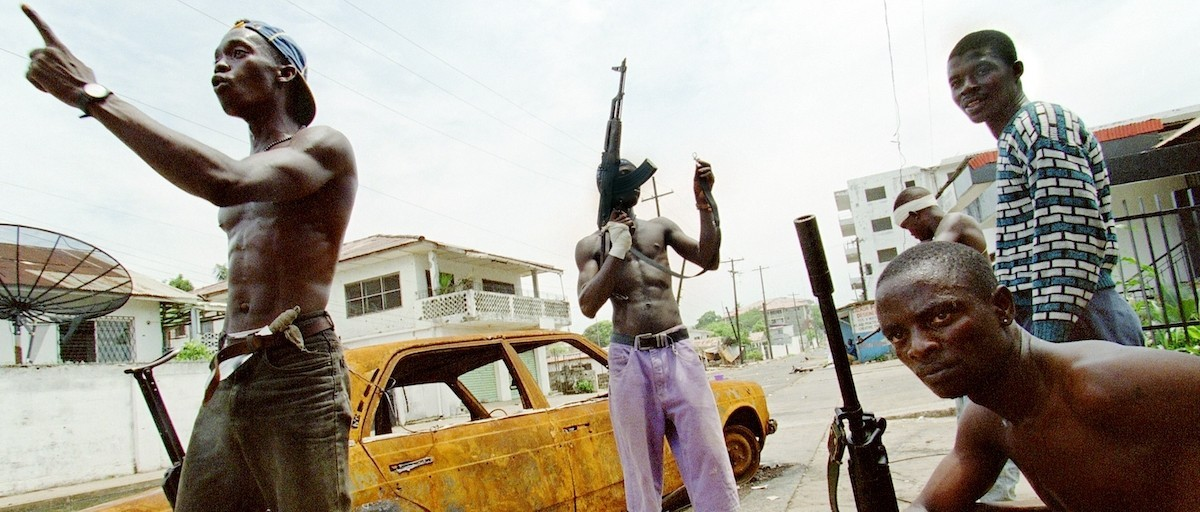
\includegraphics[width = \textwidth]{img/liberia}

Liberian Civil War

\end{frame}
% ----------------------------------------------------

% ----------------------------------------------------
\begin{frame}
\frametitle{Civil wars}
\centering

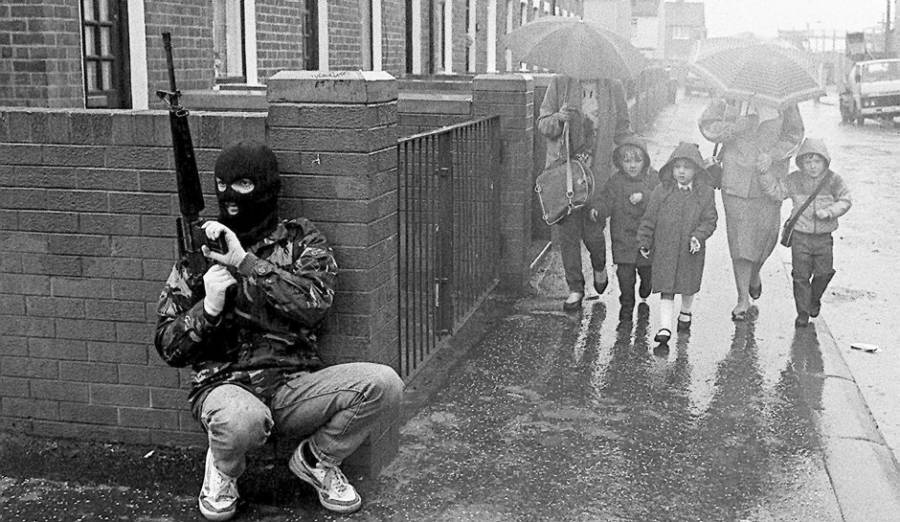
\includegraphics[width = \textwidth]{img/troubles}

Troubles, Northern Ireland

\end{frame}
% ----------------------------------------------------

% ----------------------------------------------------
\begin{frame}
\frametitle{Civil wars}
\centering

\begin{minipage}{0.49\textwidth}\centering
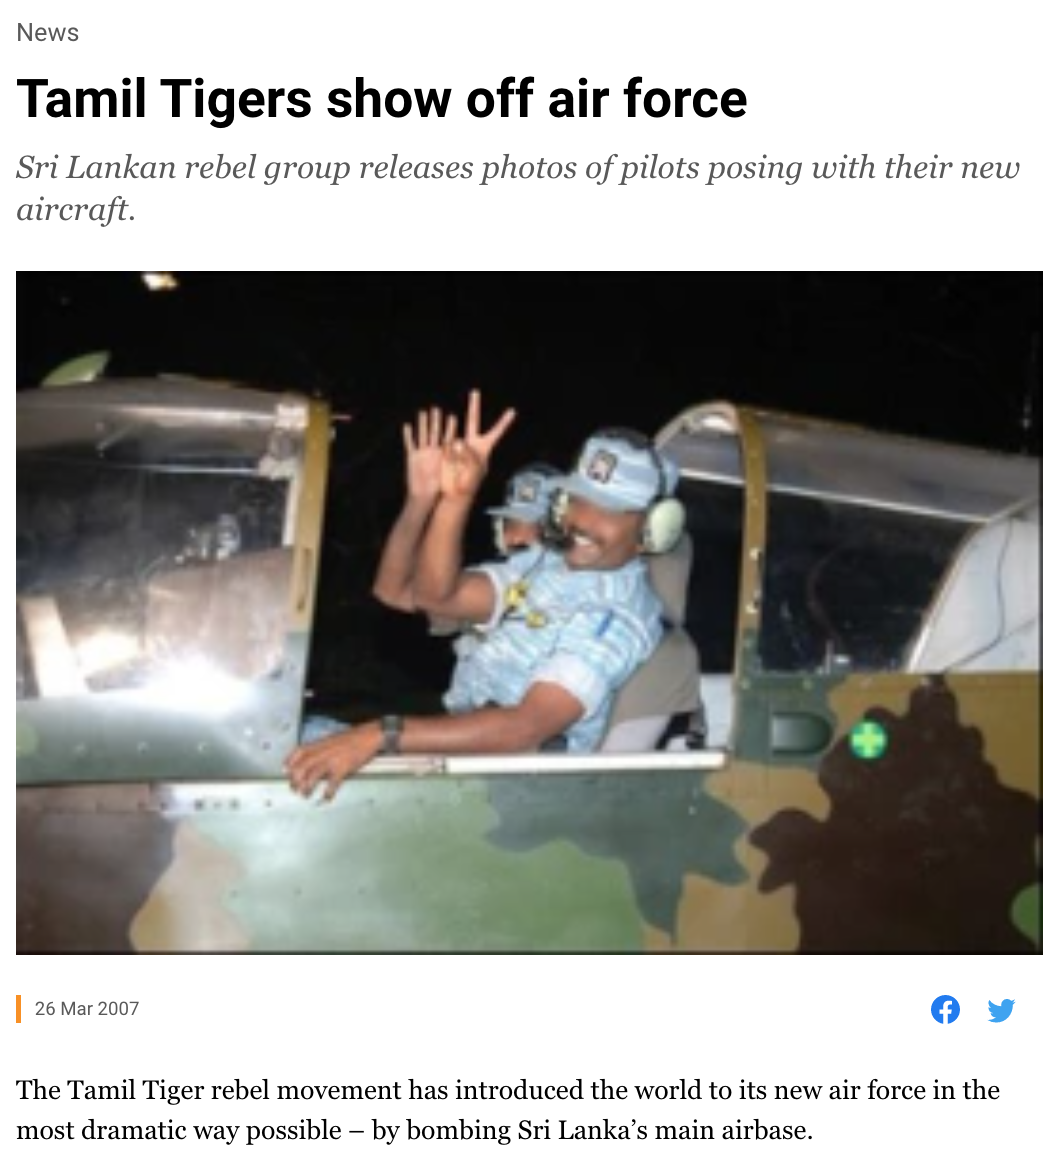
\includegraphics[width = \textwidth]{img/tigers}
\end{minipage}\hfill
\begin{minipage}{0.49\textwidth}\centering
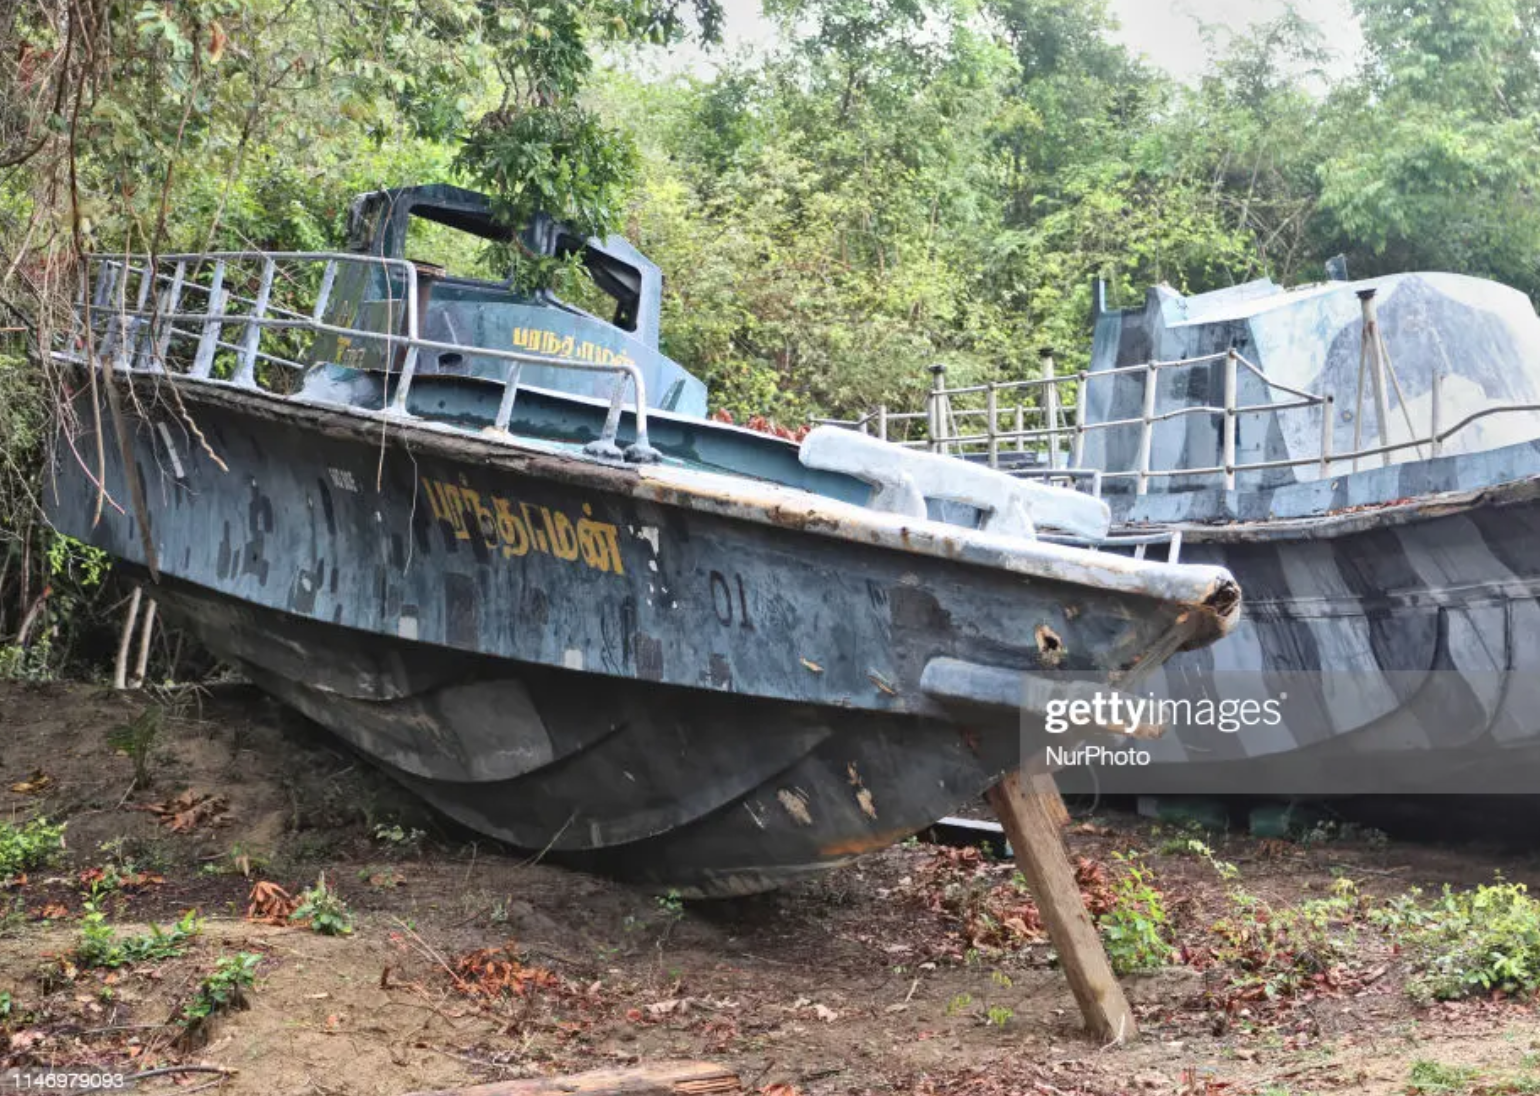
\includegraphics[width = \textwidth]{img/tigersnavy}
\end{minipage}

Sri Lankan war

\end{frame}
% ----------------------------------------------------

% ----------------------------------------------------
\begin{frame}
\frametitle{Civil Wars}
\centering

\begin{minipage}{0.49\textwidth}\centering
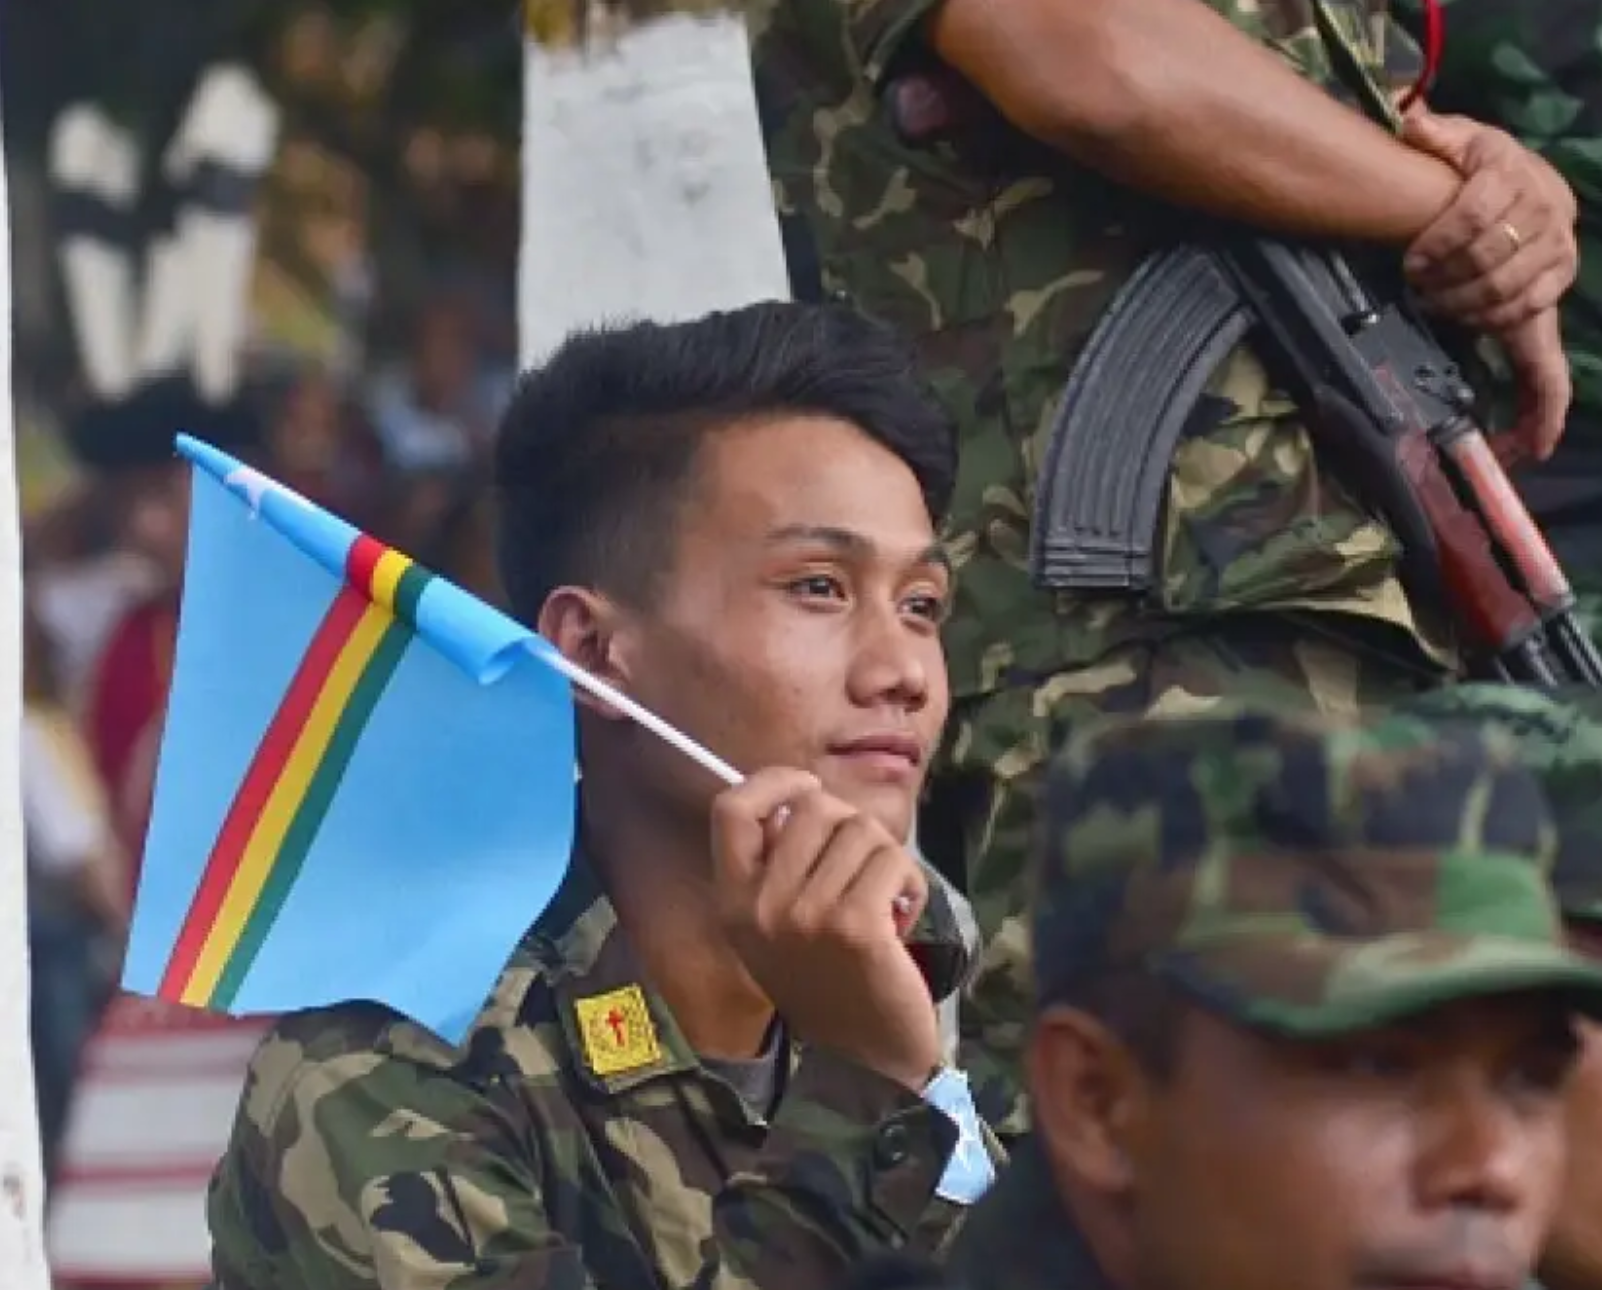
\includegraphics[width = \textwidth]{img/naga1}
\end{minipage}\hfill
\begin{minipage}{0.49\textwidth}\centering
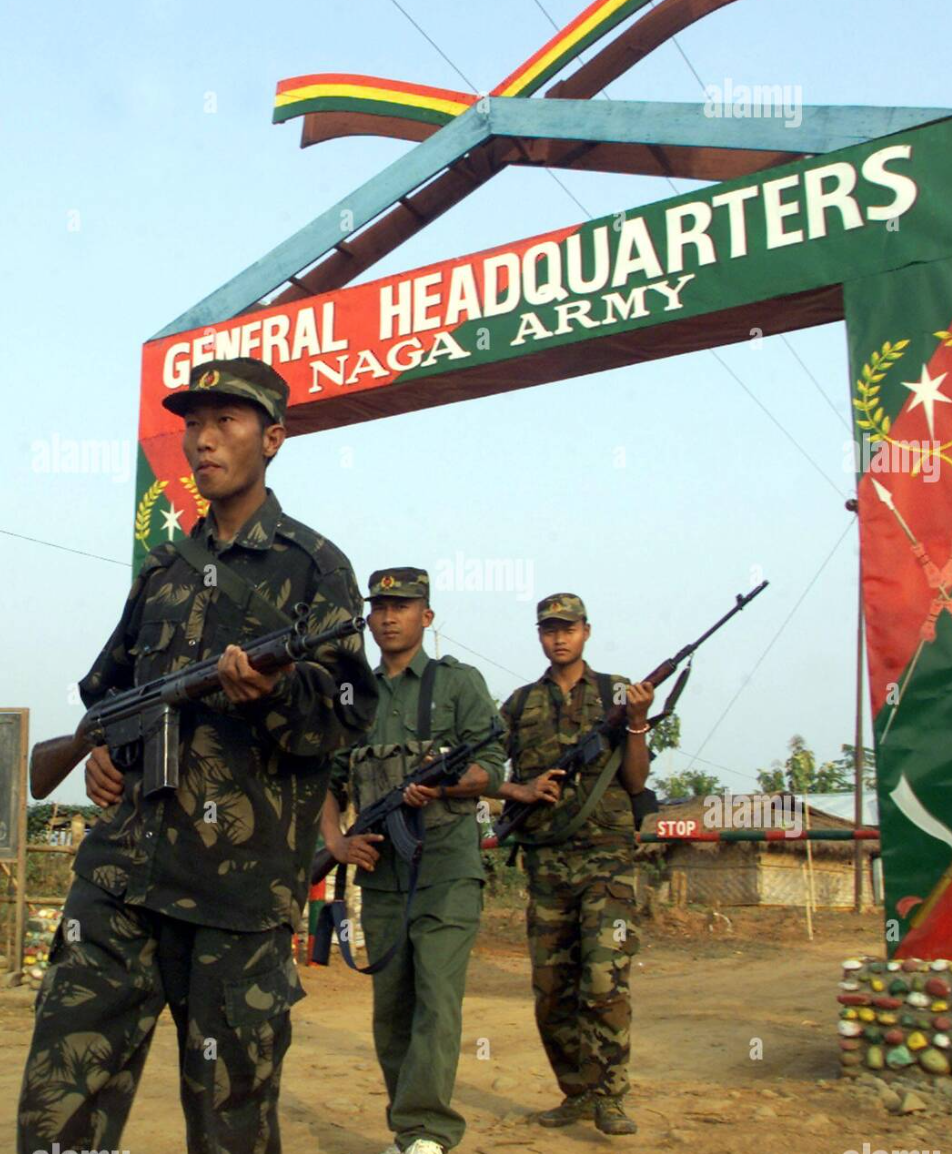
\includegraphics[width = \textwidth]{img/naga2}
\end{minipage}

Nagaland conflict, India

\end{frame}
% ----------------------------------------------------

% ----------------------------------------------------
\begin{frame}
\frametitle{Civil wars}
\centering

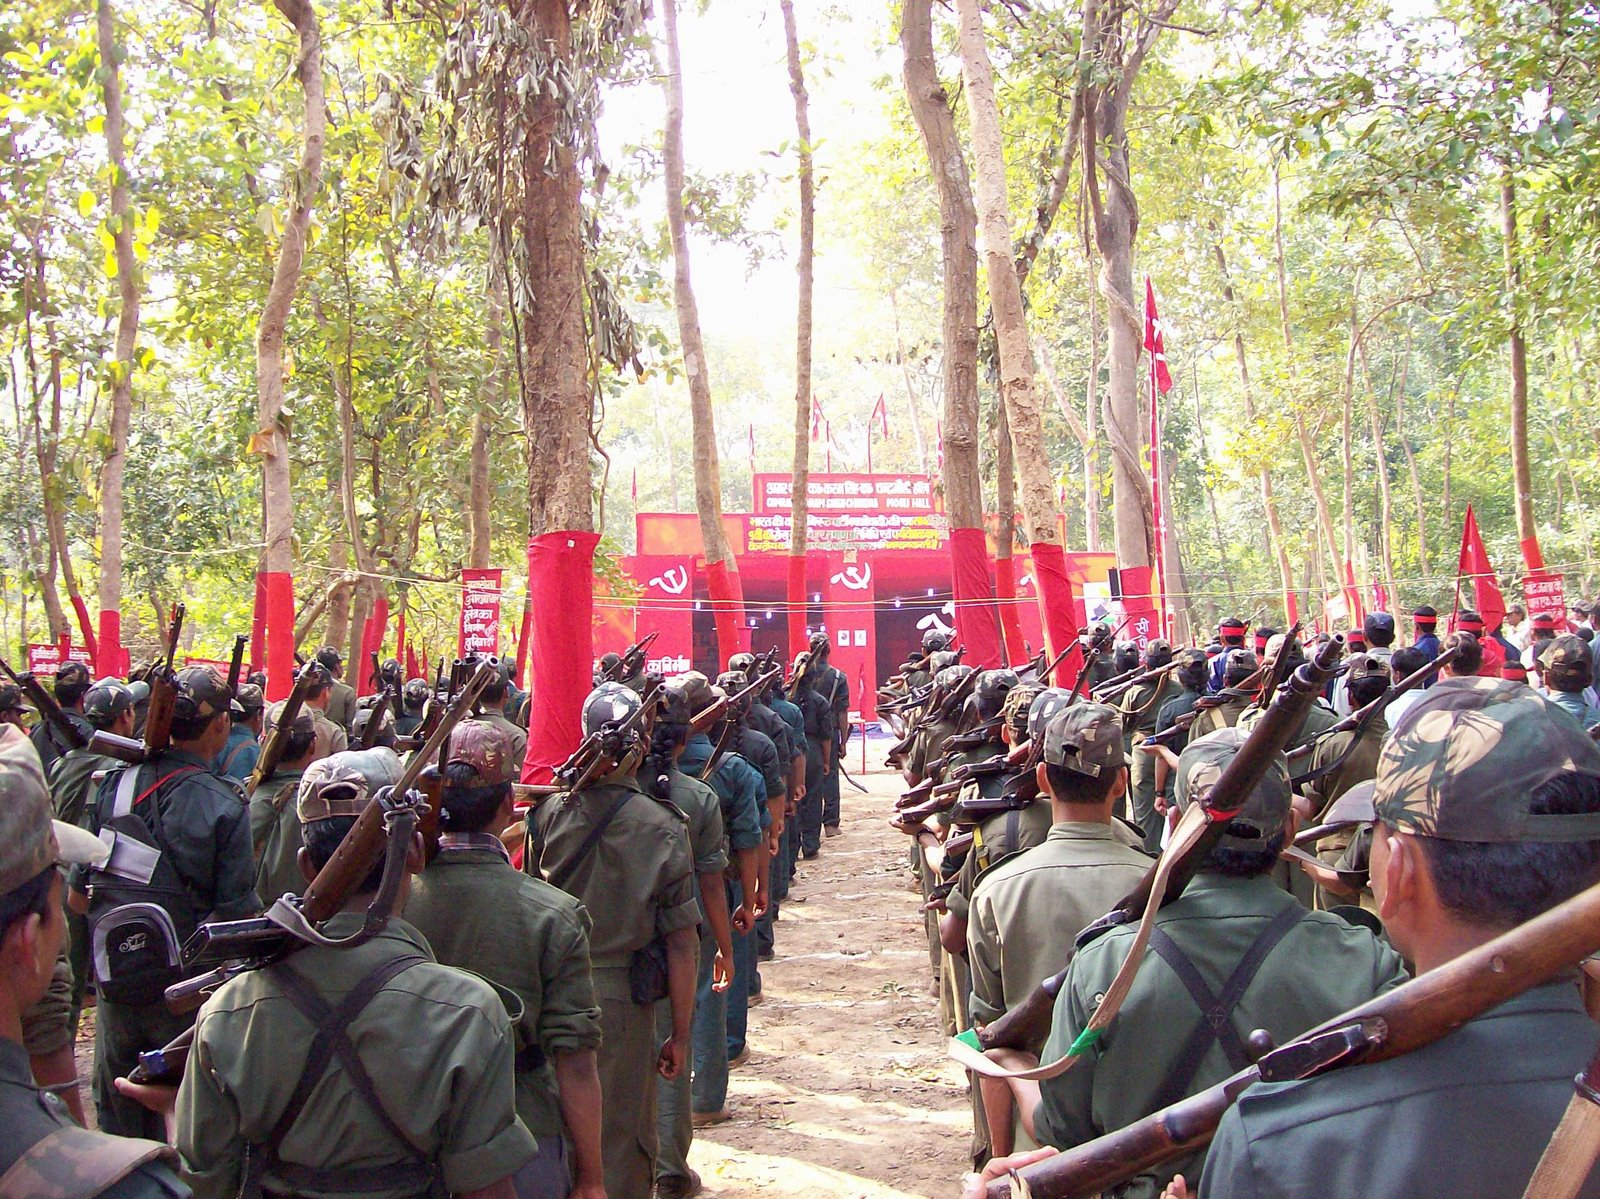
\includegraphics[width = 0.8\textwidth]{img/naxalites}

Naxalites, India

\end{frame}
% ----------------------------------------------------

% ----------------------------------------------------
\begin{frame}
\frametitle{Civil wars}
\centering

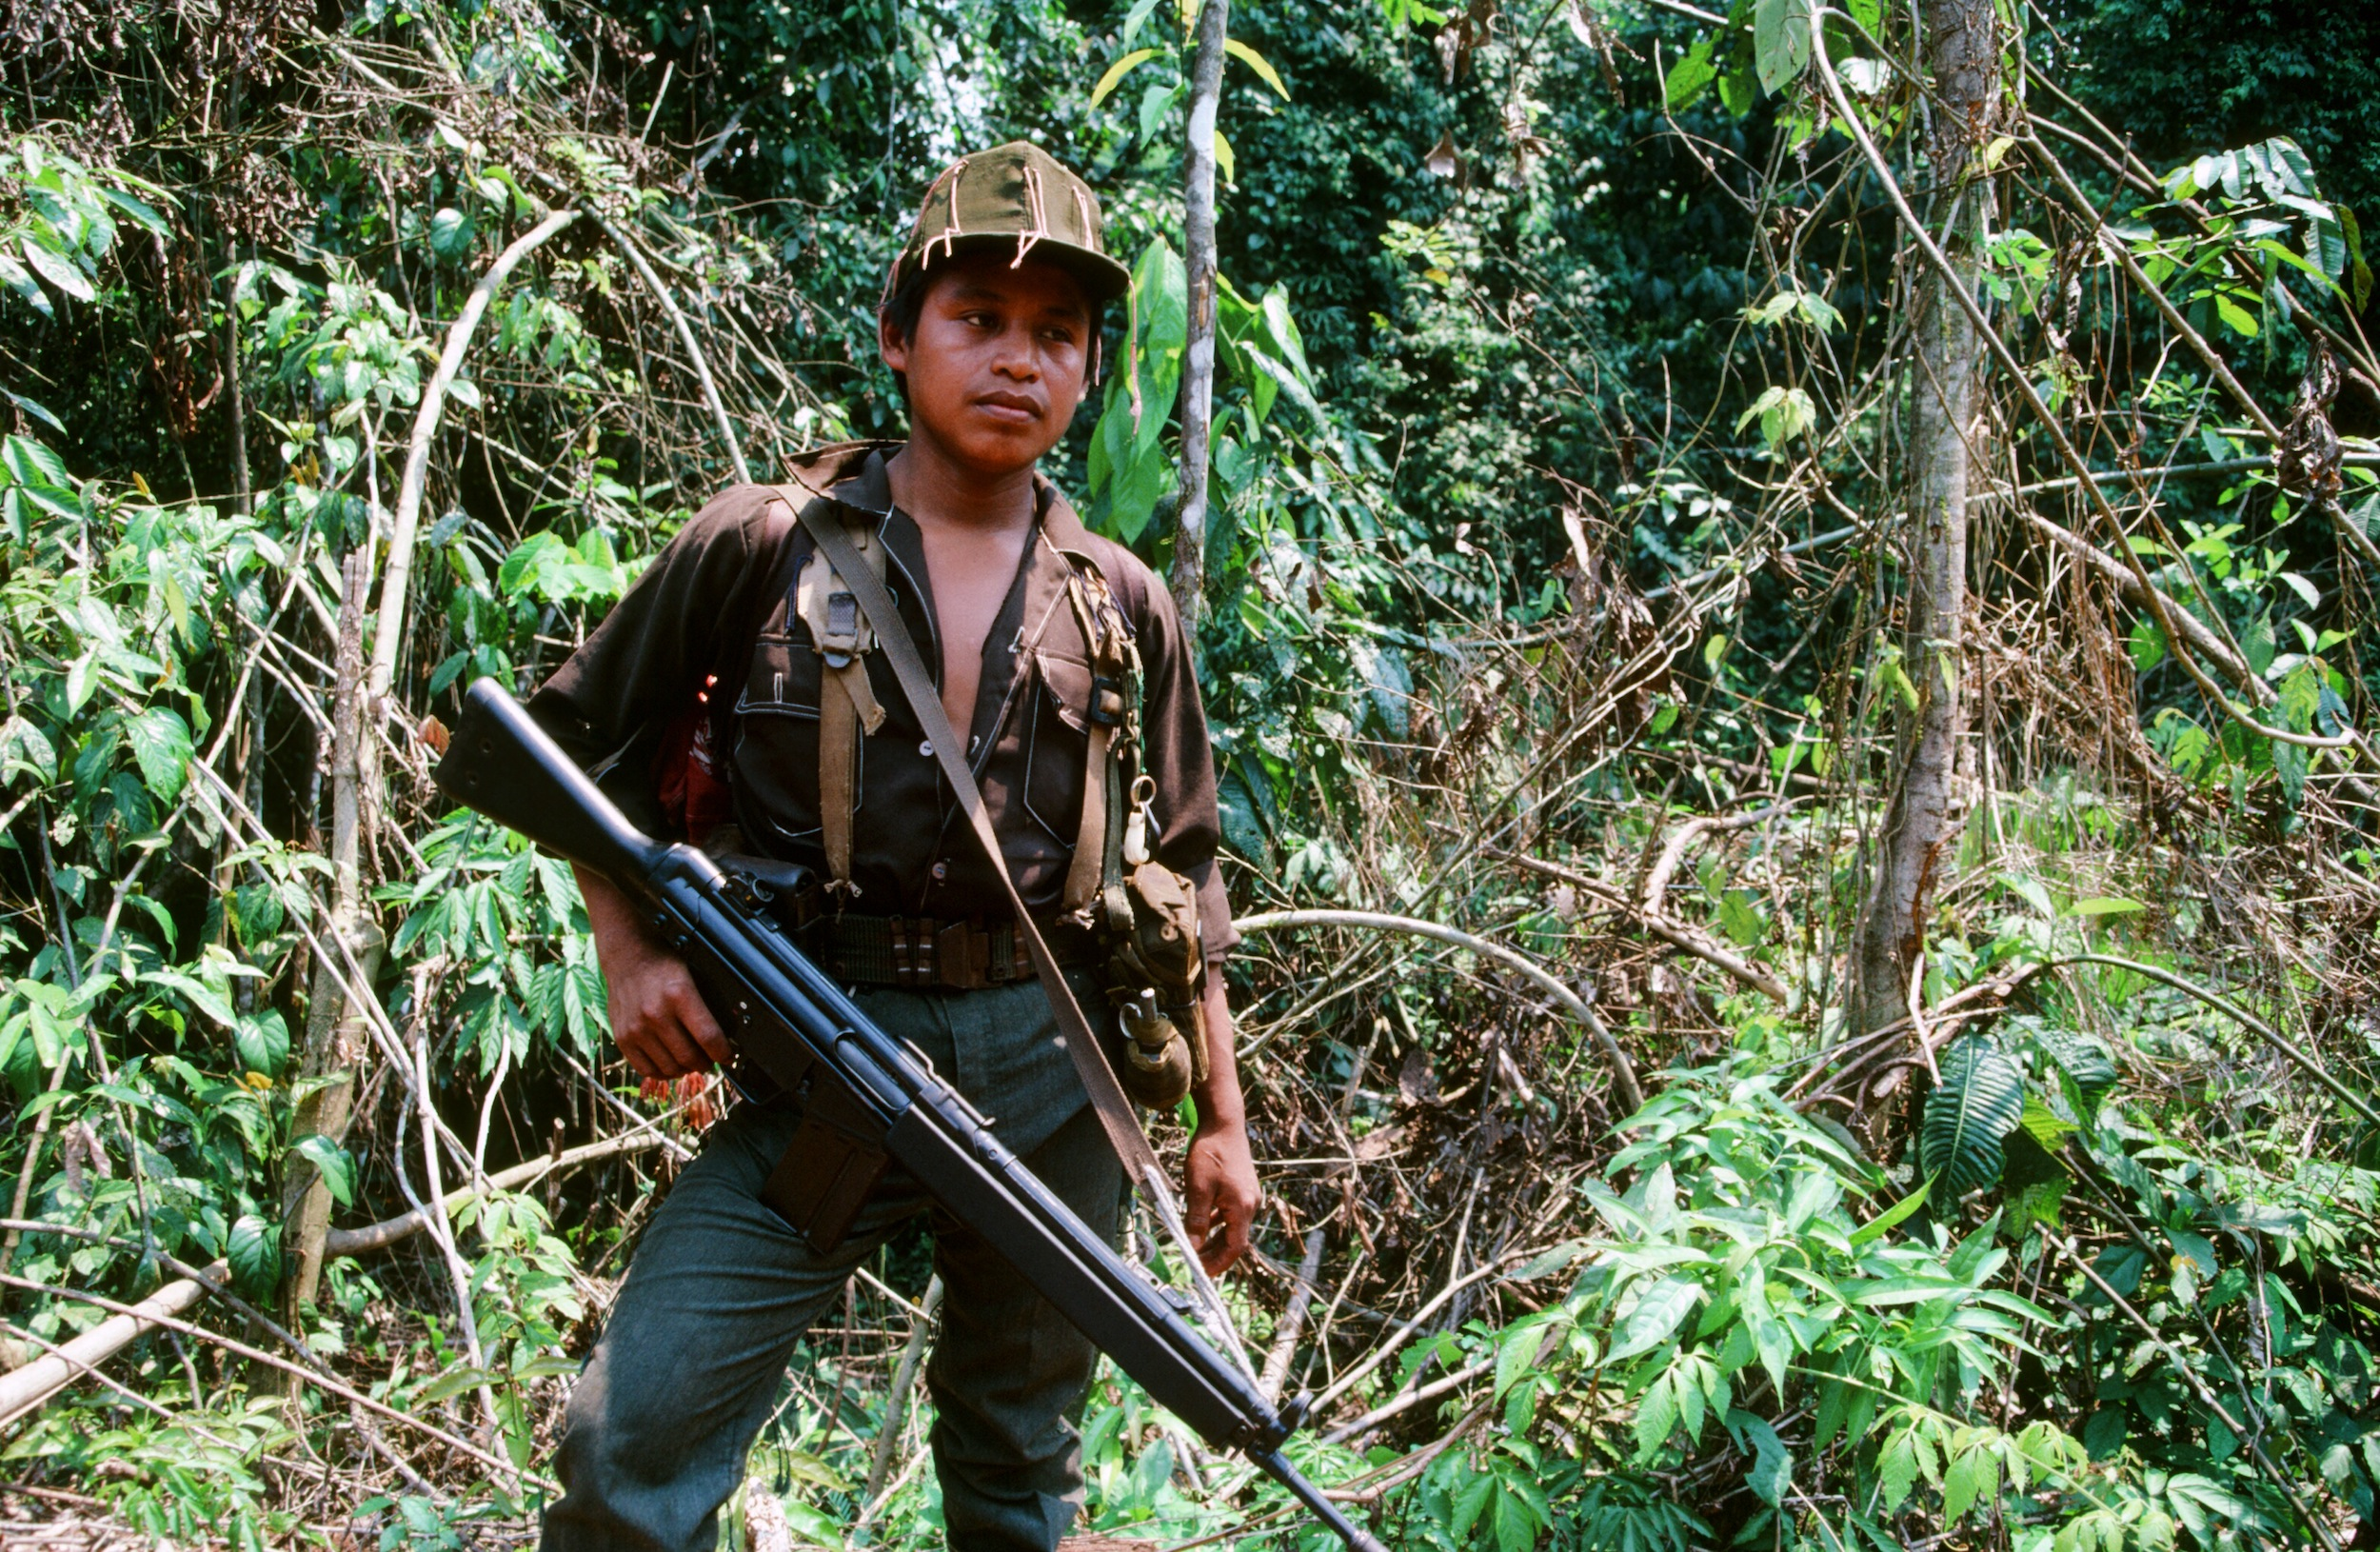
\includegraphics[width = 0.9\textwidth]{img/ixcan1988}

Guatemala

\end{frame}
% ----------------------------------------------------


% ----------------------------------------------------
\begin{frame}
\frametitle{So what is a civil war?}
\centering

\begin{itemize}
  \item What do all these have in common? And differences?
\end{itemize}

\end{frame}
% ----------------------------------------------------

% ----------------------------------------------------
\begin{frame}
\frametitle{So what is a civil war?}
\centering

\begin{itemize}
  \item Basic idea: armed conflict \textit{within} a sovereign state, fought between the government and a non-state challenger over opposite claims to sovereignty
  \begin{itemize}
    \item We usually refer to the challengers as \textit{rebel groups}
  \end{itemize}
  \item What is it that they fight over?
  \begin{itemize}
    \item Governmental civil wars: full control of the state
    \item Territorial civil wars: control over one part of the territory
  \end{itemize}
  \item Who is involved?
  \begin{itemize}
    \item Internationalized civil wars: involvement of third-party countries through alliances with local actors
  \end{itemize}
  \item How is the fighting?
  \begin{itemize}
    \item Warfare technology
  \end{itemize}
\end{itemize}

\end{frame}
% ----------------------------------------------------

% ----------------------------------------------------
\begin{frame}
\frametitle{Technologies of rebellion}
\centering

\begin{itemize}
  \item Not all rebel groups look the same
  \item Some actually don't even look like rebel groups (or the idea we usually have of them)
  \begin{itemize}
    \item e.g. Confederate States, Franco's Nationalists
  \end{itemize}
  \item Same applies sometimes to the government forces
  \item Concept: technologies of rebellion
  \begin{itemize}
    \item What kind of fighting forces are the rebels capable of launching?
    \item Guerrillas? Conventional armies?
  \end{itemize}
\end{itemize}

\end{frame}
% ----------------------------------------------------

% ----------------------------------------------------
\begin{frame}
\frametitle{Technologies of rebellion}
\centering

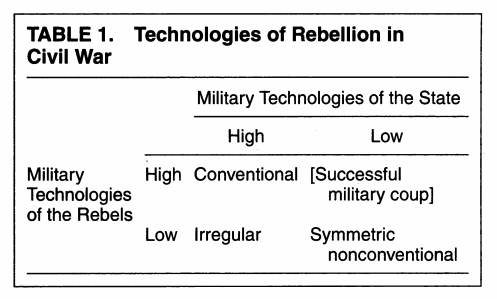
\includegraphics[width = 0.8\textwidth]{img/kalyvas_balcells_tr}\\
{\small Balcells \& Kalyvas (\textit{APSR} 2010)}

\end{frame}
% ----------------------------------------------------

% ----------------------------------------------------
\begin{frame}
\frametitle{Technologies of rebellion}
\centering

\begin{itemize}
  \item Irregular wars
  \begin{itemize}
    \item[] $\approx$ 34\% (1944--2004)
    \item[] (e.g. Nepal, Peru, etc)
  \end{itemize}
  \item Conventional wars
  \begin{itemize}
    \item[] $\approx$ 54\%
    \item[] (e.g. US, Spain, Sri Lanka, Syria)
  \end{itemize}
  \item Symmetric non-conventional
  \begin{itemize}
    \item[] $\approx$ 12\%
    \item[] (Somalia, CAR)
  \end{itemize}
\end{itemize}

\end{frame}
% ----------------------------------------------------

% ----------------------------------------------------
\begin{frame}
\frametitle{What is \BGyellow{not} a civil war?}
\centering

\begin{itemize}
\setbeamercovered{transparent}
  \item<1> It's \textit{not} violence against civilians
  \begin{itemize}
    \item War $\neq$ violence
  \end{itemize}
  \item<2> It's \textit{not} terrorism
  \begin{itemize}
    \item Although terrorism can be used within wars
  \end{itemize}
  \item<3> It's \textit{not} genocide
  \begin{itemize}
    \item Any war involves sustained, bidirectional battle violence
  \end{itemize}
  \item<4> It's \textit{not} non-state violence (e.g. communal riots)
  \begin{itemize}
    \item State/government is always one participant
  \end{itemize}
  \item<5> It's \textit{not} ethnic conflict
  \begin{itemize}
    \item Although there are \textit{ethnic} civil wars (but ethnic conflict also includes ethnic riots, or ethnic violence against civilians)
  \end{itemize}
\end{itemize}

\end{frame}
% ----------------------------------------------------

% ----------------------------------------------------
\begin{frame}
\frametitle{Patterns of conflicts over time}
\centering

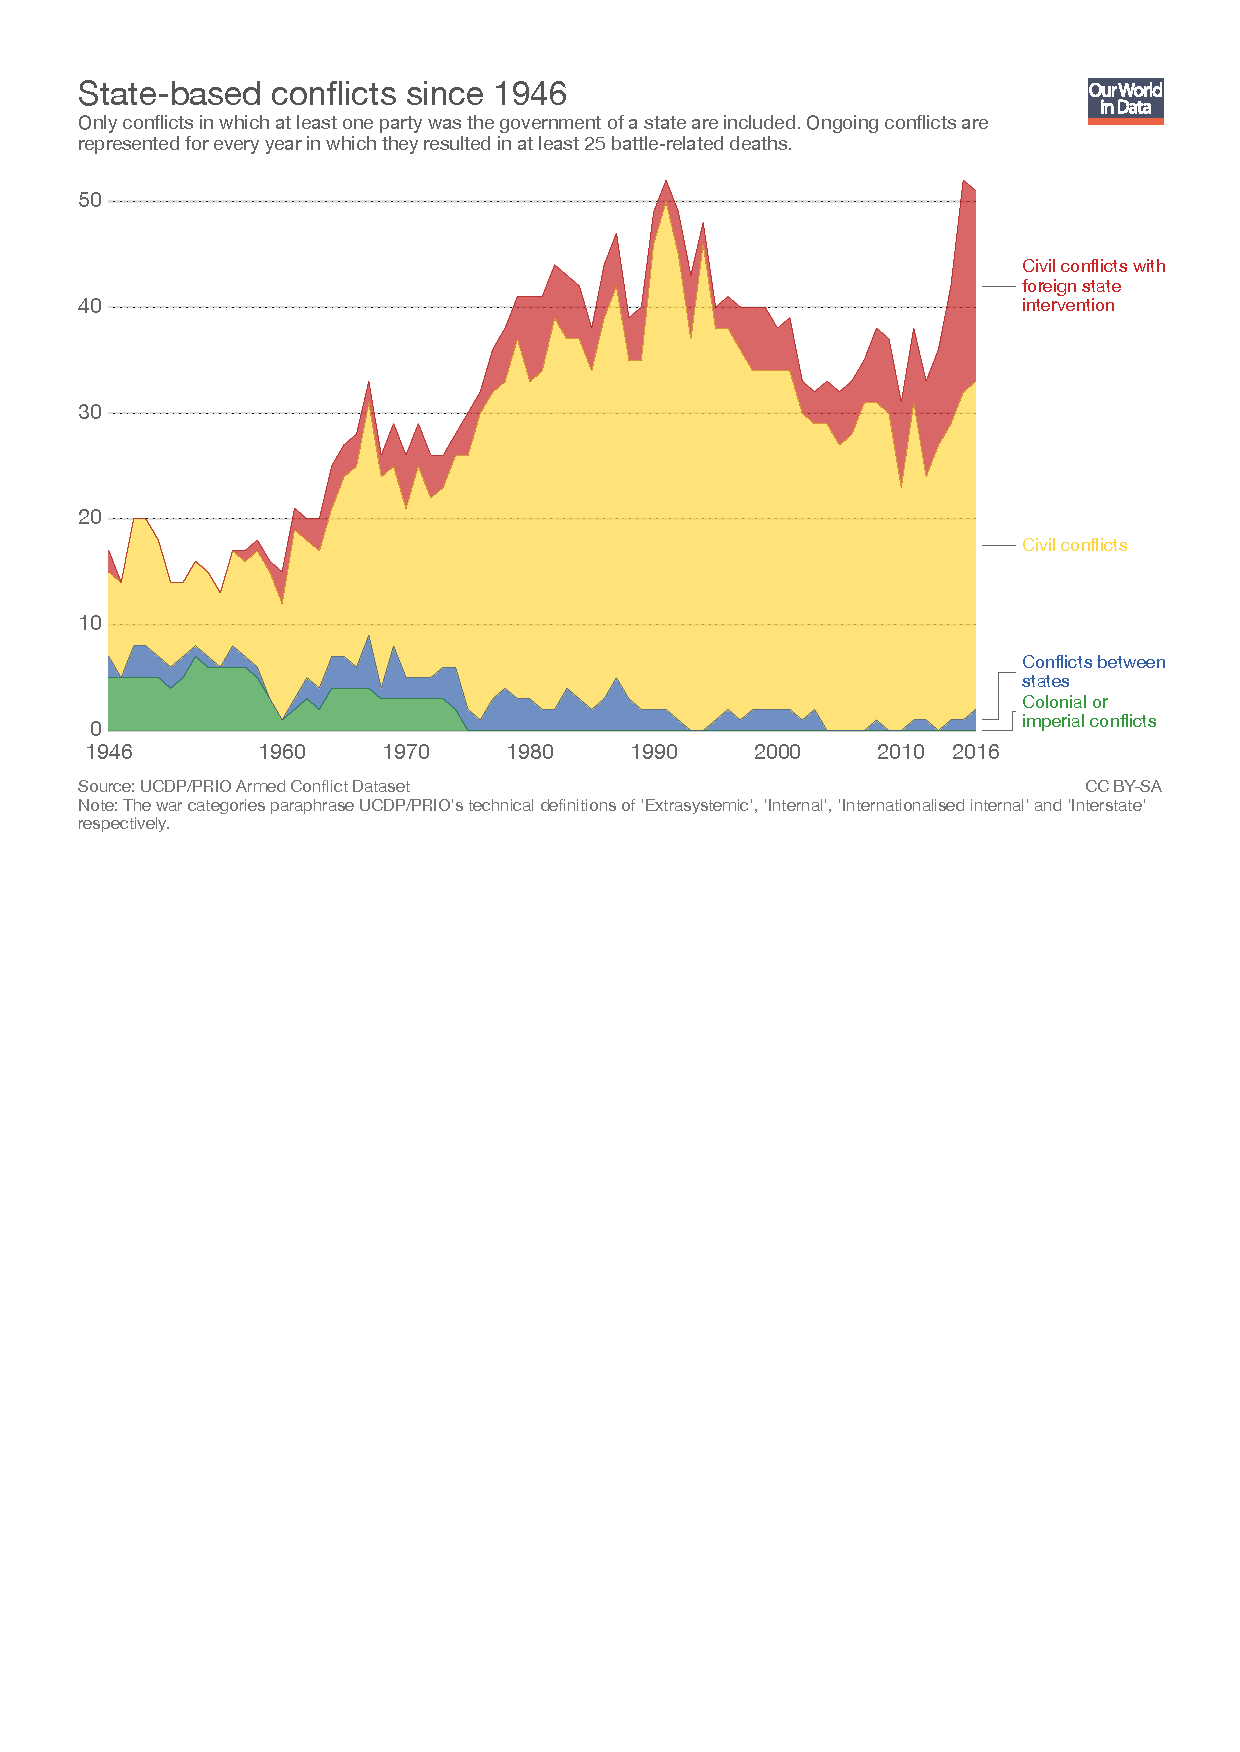
\includegraphics[width = 0.9\textwidth]{img/conflicts_over_time}

{\small \textit{Source:} UCDP-PRIO \& \url{https://ourworldindata.org/}}

\end{frame}
% ----------------------------------------------------

% ----------------------------------------------------
\begin{frame}
\frametitle{Patterns of conflicts over time}
\centering

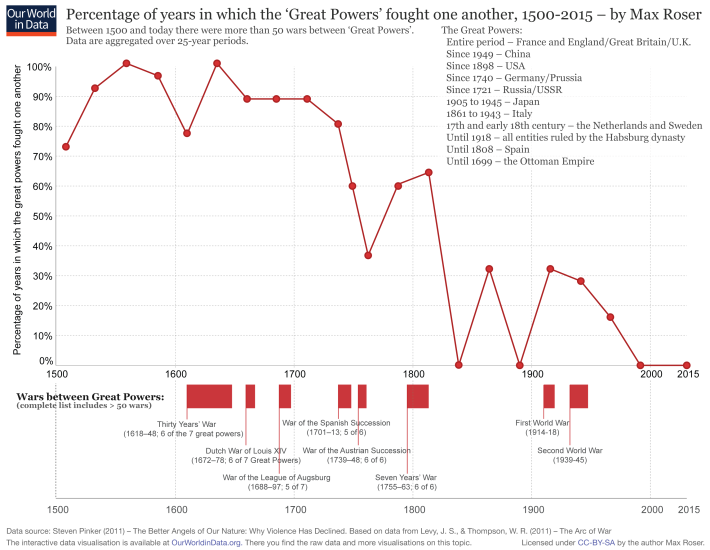
\includegraphics[width = 0.85\textwidth]{img/great_powers_wars}

{\small \textit{Source:} UCDP-PRIO \& \url{https://ourworldindata.org/}}

\end{frame}
% ----------------------------------------------------

% ----------------------------------------------------
\begin{frame}
\frametitle{What do we know about civil wars?}
\centering

\begin{itemize}
  \item<1-> \BGyellow{Onset of civil wars}
  \begin{itemize}
    \item Why, where and when do they break out?
  \end{itemize}
  \item<2-> \textbf{Wartime dynamics}
  \begin{itemize}
    \item What happens during a civil war? How do we explain wartime violence?
  \end{itemize}
  \item<3-> \textbf{Termination of civil wars}
  \begin{itemize}
    \item How and when do they end?
  \end{itemize}
  \item<4-> \textbf{Postwar politics}
  \begin{itemize}
    \item How do we avoid the relapse of civil wars? What are their consequences?
    \item The `conflict trap'
  \end{itemize}
\end{itemize}

\end{frame}
% ----------------------------------------------------

% ----------------------------------------------------
\begin{frame}
\frametitle{Understanding civil wars}
\centering

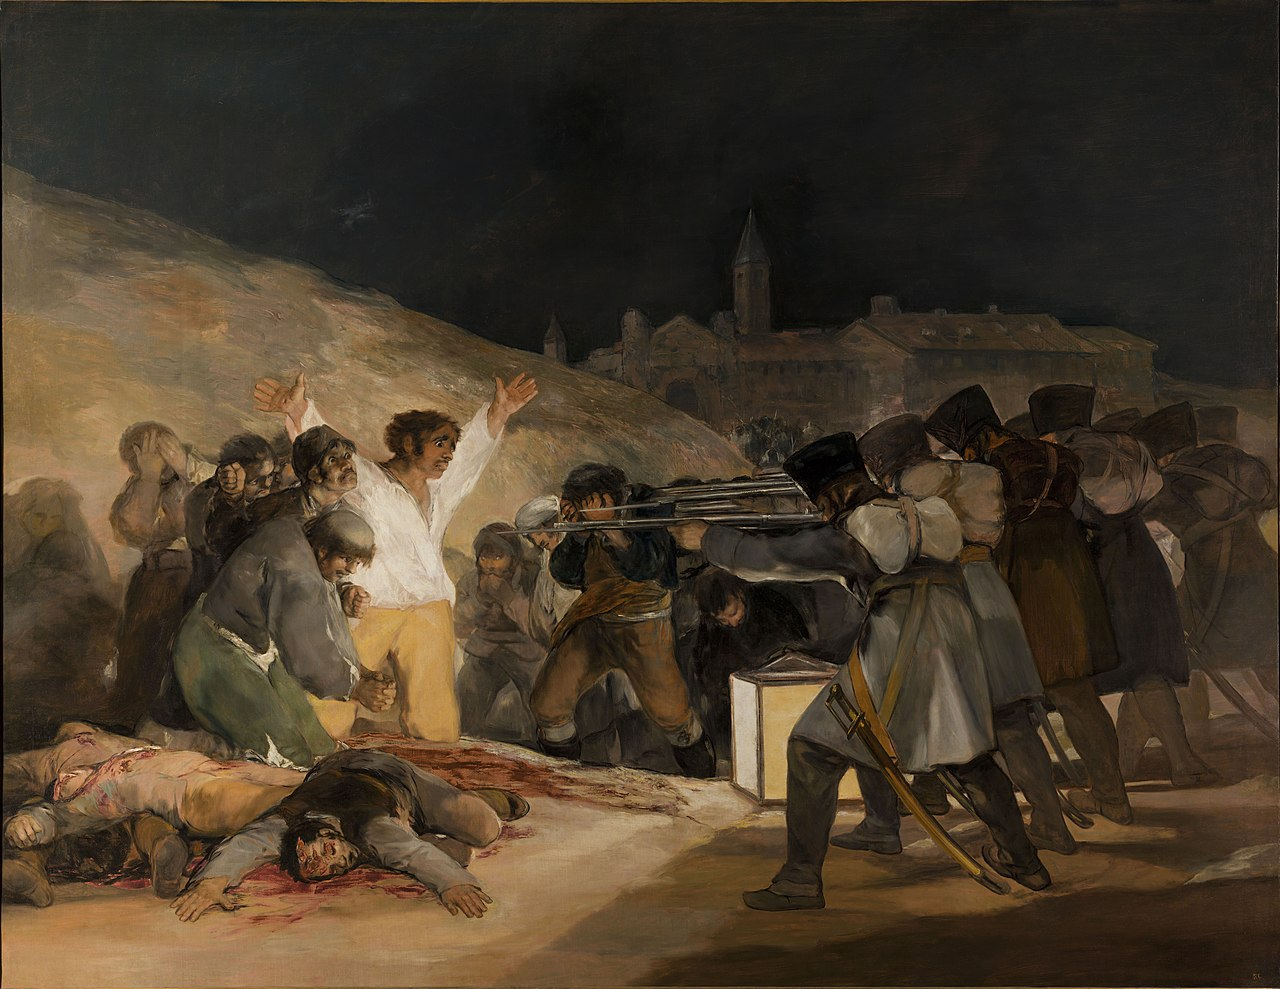
\includegraphics[width = \textwidth]{img/goya}

\textit{Duelo a garrotazos} (Goya, ca. 1820)

\vspace{15pt}

\begin{itemize}
  \item Civil wars were traditionally seen as irrational mass violence
\end{itemize}

\end{frame}
% ----------------------------------------------------

% ----------------------------------------------------
\begin{frame}
\frametitle{Context}
\centering

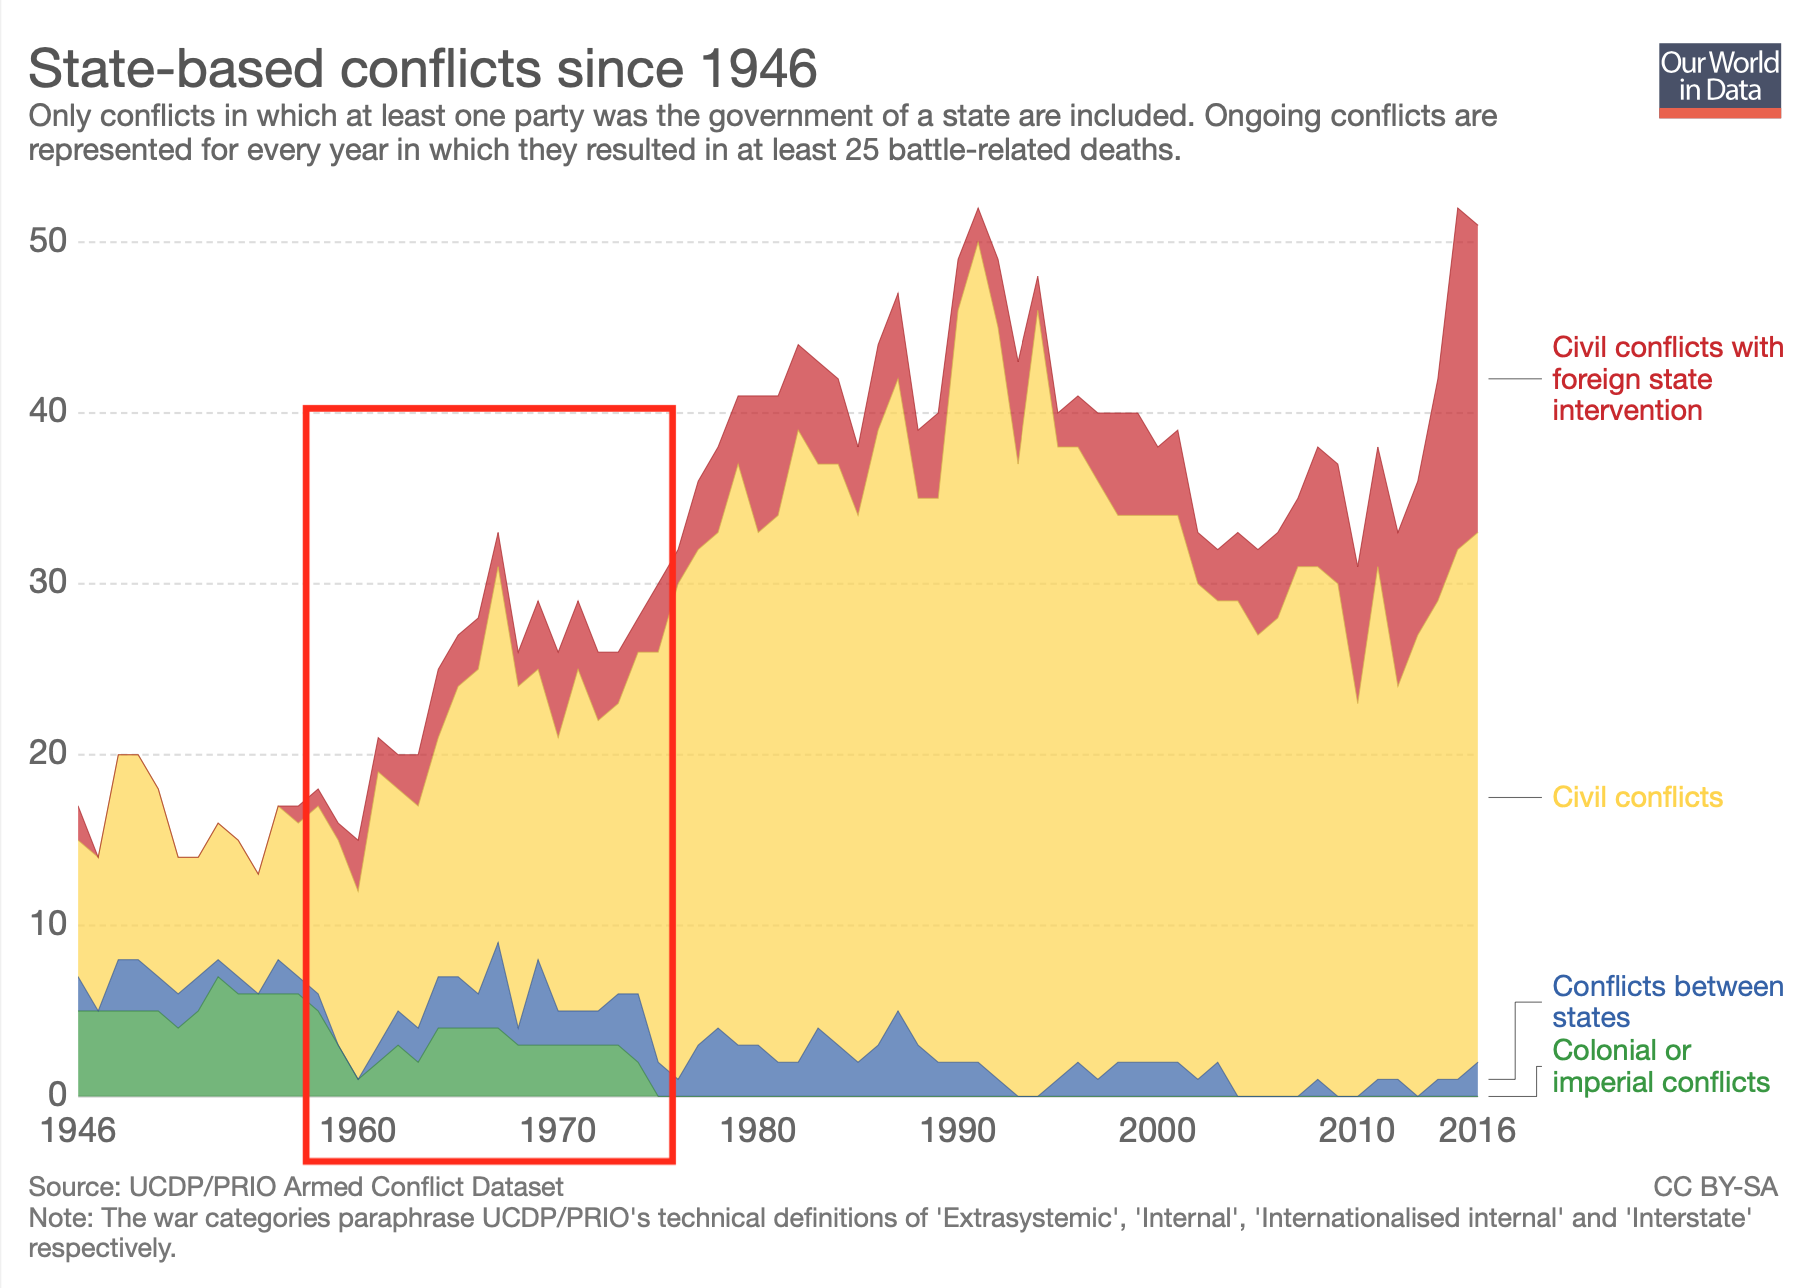
\includegraphics[width = 0.8\textwidth]{img/conflicts_over_time2}

\begin{itemize}
  \item Increase of civil war incidence after the 1960s
\end{itemize}

\end{frame}
% ----------------------------------------------------

% ----------------------------------------------------
\begin{frame}
\frametitle{Context}
\centering

\begin{minipage}{0.58\textwidth}\centering
\begin{itemize}
  \item Role of decolonization from 1960 on
  \item Newly independent countries followed Western-style form of state rule
  \begin{itemize}
    \item Centralized administrations, clear territorial borders (e.g. Organisation of African Unity, Addis Ababa, 1963)
  \end{itemize}
  \item<2-> But clear \BGyellow{problems of state capacity}
\end{itemize}
\end{minipage}\hfill
\begin{minipage}{0.4\textwidth}\centering
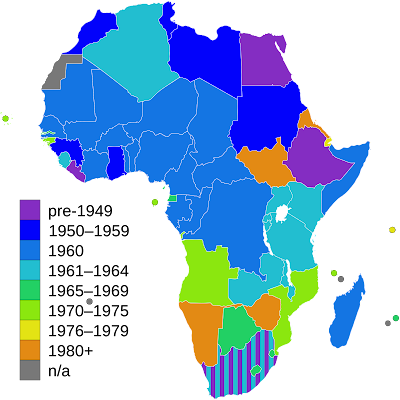
\includegraphics[width = \textwidth]{img/africa_decolonization}\\
Decolonization in Africa
\end{minipage}

\end{frame}
% ----------------------------------------------------

% ----------------------------------------------------
\begin{frame}
\frametitle{Context}
\centering

\begin{minipage}{0.58\textwidth}\centering
\begin{itemize}
  \item Spread of \BGyellow{revolutionary insurgencies}
  \item Role of ideological global context
  \begin{itemize}
    \item Cold War and US/USSR rivalry
  \end{itemize}
\end{itemize}
\end{minipage}\hfill
\begin{minipage}{0.4\textwidth}\centering
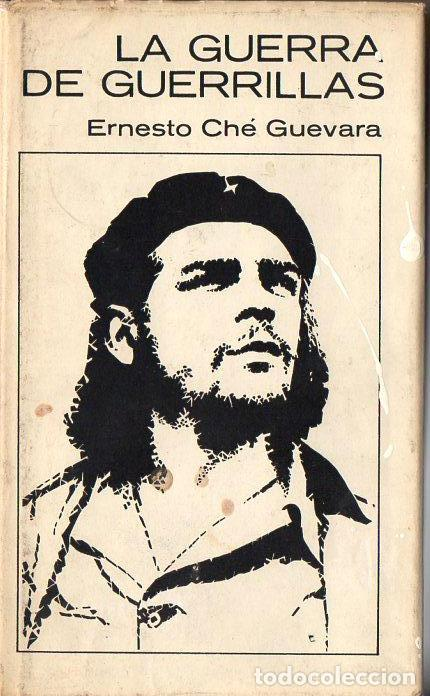
\includegraphics[width = 0.9\textwidth]{img/guevara}
\end{minipage}

\end{frame}
% ----------------------------------------------------

% ----------------------------------------------------
\begin{frame}
\frametitle{Early studies}
\centering

\begin{minipage}{0.59\textwidth}\centering
\begin{itemize}
  \item Early studies on \BGyellow{revolutions}
  \item Focus on grievances, inequality
  \item That was the prevailing way of studying this before the 1990s
  \item Even if they were \textbf{not studied as} `civil wars,' but as `\textbf{peasant rebellions}' or `\textbf{social revolutions}'
  \begin{itemize}
    \item Mixing onset with outcome, etc
  \end{itemize}
\end{itemize}
\end{minipage}\hfill
\begin{minipage}{0.39\textwidth}\centering
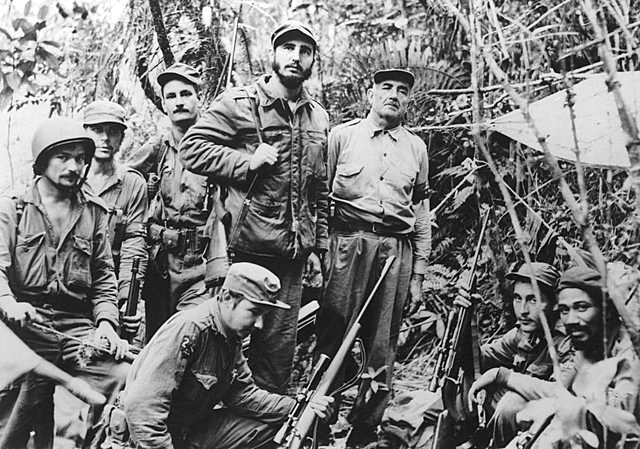
\includegraphics[width = \textwidth]{img/cuban}\\Cuban Revolution
\end{minipage}

\end{frame}
% ----------------------------------------------------

% ----------------------------------------------------
\begin{frame}
\frametitle{Early studies}
\centering

\begin{minipage}{0.59\textwidth}\centering
  \begin{itemize}
    \item Things started to change in the 1990s
    \item The end of the Cold War
    \item Yugoslavia, Rwanda and the role of ethnicity
    \item Ancient hatreds, `clash of civilizations', etc
  \end{itemize}
\end{minipage}\hfill
\begin{minipage}{0.39\textwidth}\centering
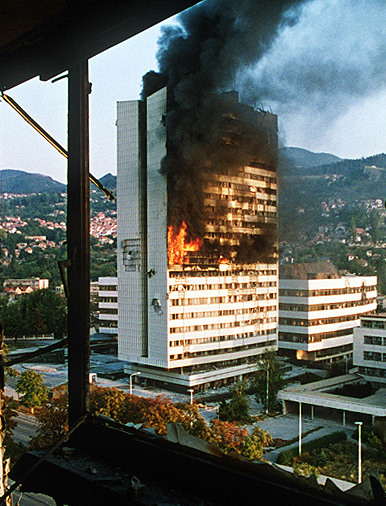
\includegraphics[width = \textwidth]{img/sarajevo}\\Siege of Sarajevo
\end{minipage}

\end{frame}
% ----------------------------------------------------

% ----------------------------------------------------
\begin{frame}
\frametitle{Research on `civil wars'}
\centering

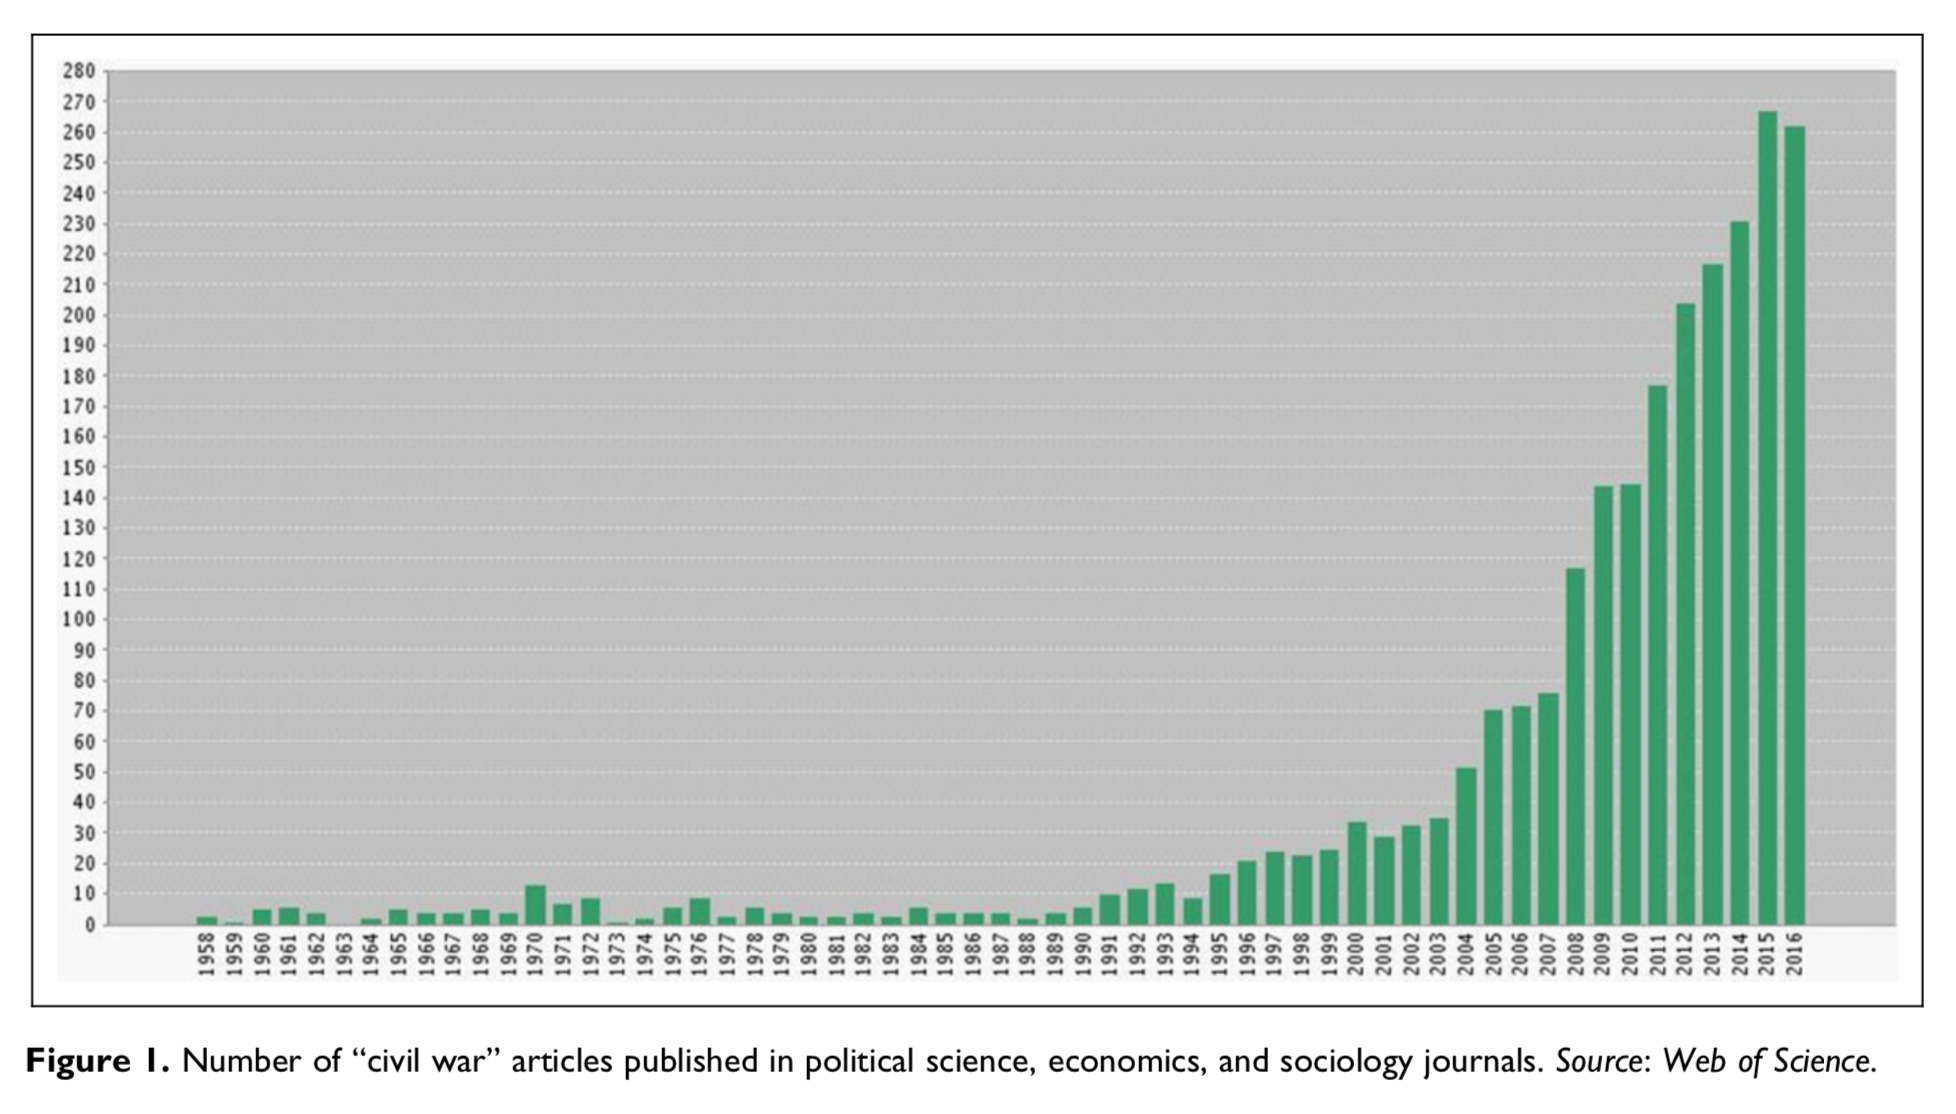
\includegraphics[width = \textwidth]{img/cw_studies}

\end{frame}
% ----------------------------------------------------

% ----------------------------------------------------
\begin{frame}
\frametitle{How it started: the role of development economists}
\centering

\begin{minipage}{0.5\textwidth}\centering
\begin{itemize}
  \item Civil wars as a development problem
  \item What drives civil wars?
  \item First quantitative analyses of CW onset
  \item New explanation: greed
  \begin{itemize}
    \item Greed vs. grievance debate
  \end{itemize}
\end{itemize}
\end{minipage}\hfill
\begin{minipage}{0.5\textwidth}\centering
\frame{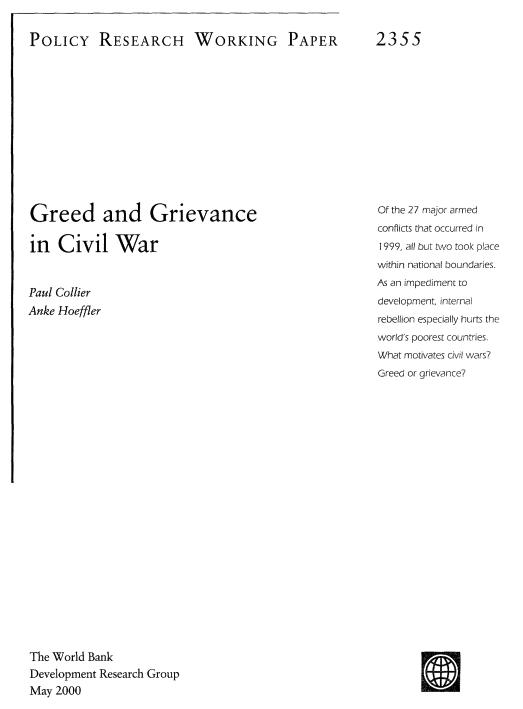
\includegraphics[width = 0.85\textwidth]{img/greed_grievance}}\\
{\small Paul Collier \& Anke Hoeffler (2000)}
\end{minipage}

\end{frame}
% ----------------------------------------------------

% ----------------------------------------------------
\begin{frame}
\frametitle{The \textit{greed} perspective}
\centering

\begin{itemize}[<+->]
  \item Previous studies on revolutions highlighted the role of grievances: peasants rise up because they are oppresed
  \item Collier \& Hoeffler argued that grievances do not explain anything because they are always present
  \item Grievances are just used by \BGyellow{greedy rebels} who think a civil war is a good opportunity to get rich
  \item \BGyellow{Microeconomic perspective}: civil wars erupt if the the opportunity cost of violence is low (poverty) and the expected gains are high (natural resources \& looting)
\end{itemize}

\end{frame}
% ----------------------------------------------------

% ----------------------------------------------------
\begin{frame}
\frametitle{Empirics in Collier \& Hoeffler model}
\centering

\begin{itemize}
  \item[] Key variables:
  \item \textbf{Male secondary schooling:} opportunity cost of joining insurgency
  \item \textbf{Primary commodity exports:} expected gains
  \item \textbf{Social fractionalization:} should capture grievances
  \item[]
  \item Analyzing determinants of onset in country-year data
\end{itemize}

\end{frame}
% ----------------------------------------------------

% ----------------------------------------------------
\begin{frame}
\frametitle{}
\centering

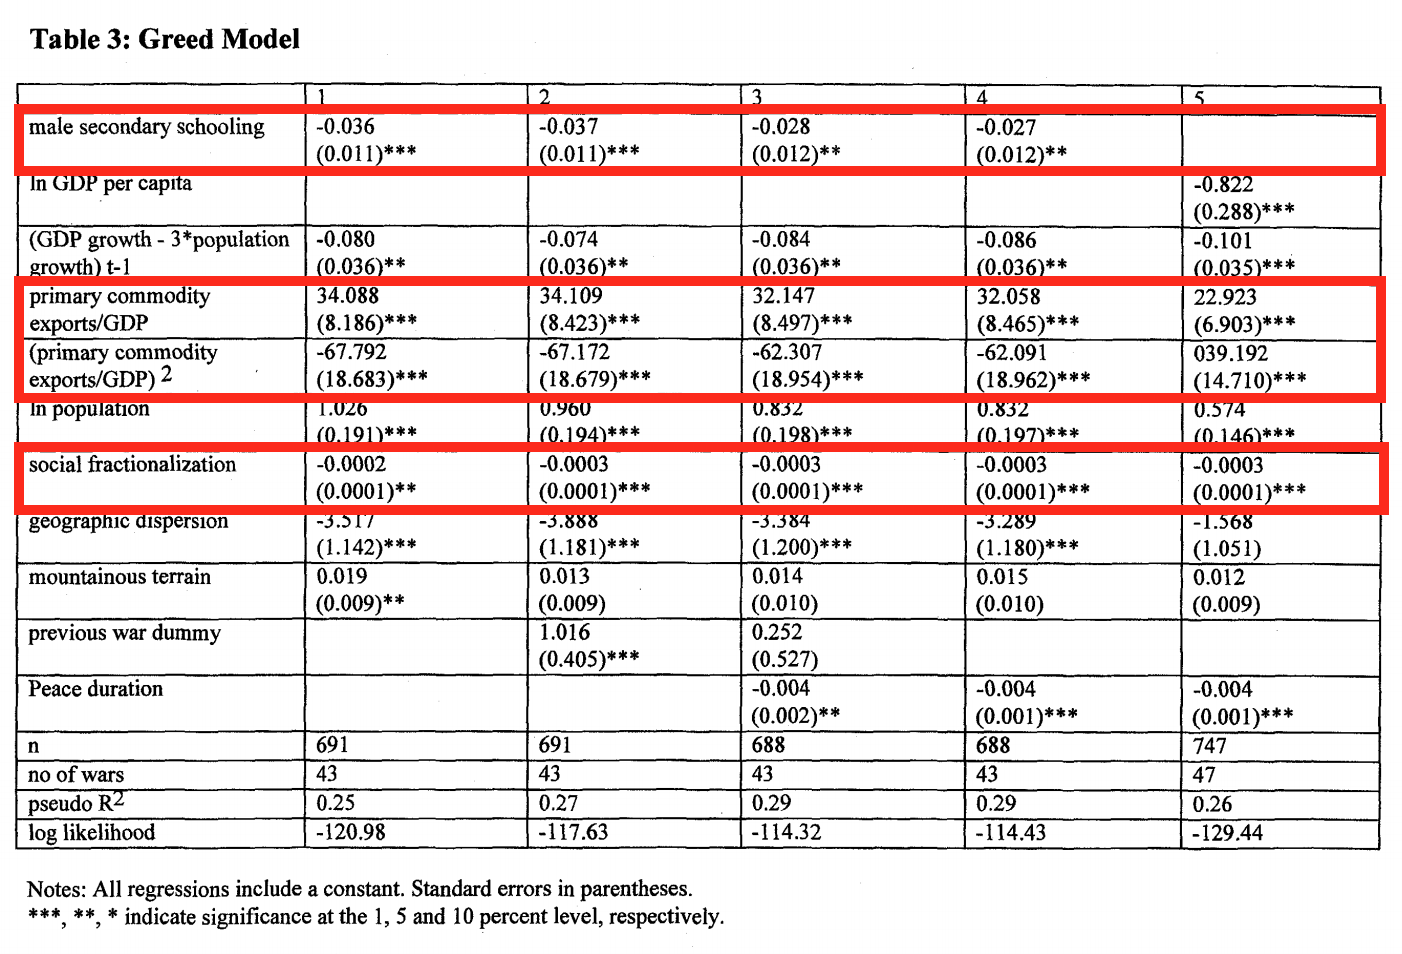
\includegraphics[width = \textwidth]{img/collier_hoeffler_model}

{\small Collier \& Hoeffler (2000)}

\end{frame}
% ----------------------------------------------------

% ----------------------------------------------------
\begin{frame}
\frametitle{The \textit{greed} perspective: context}
\centering

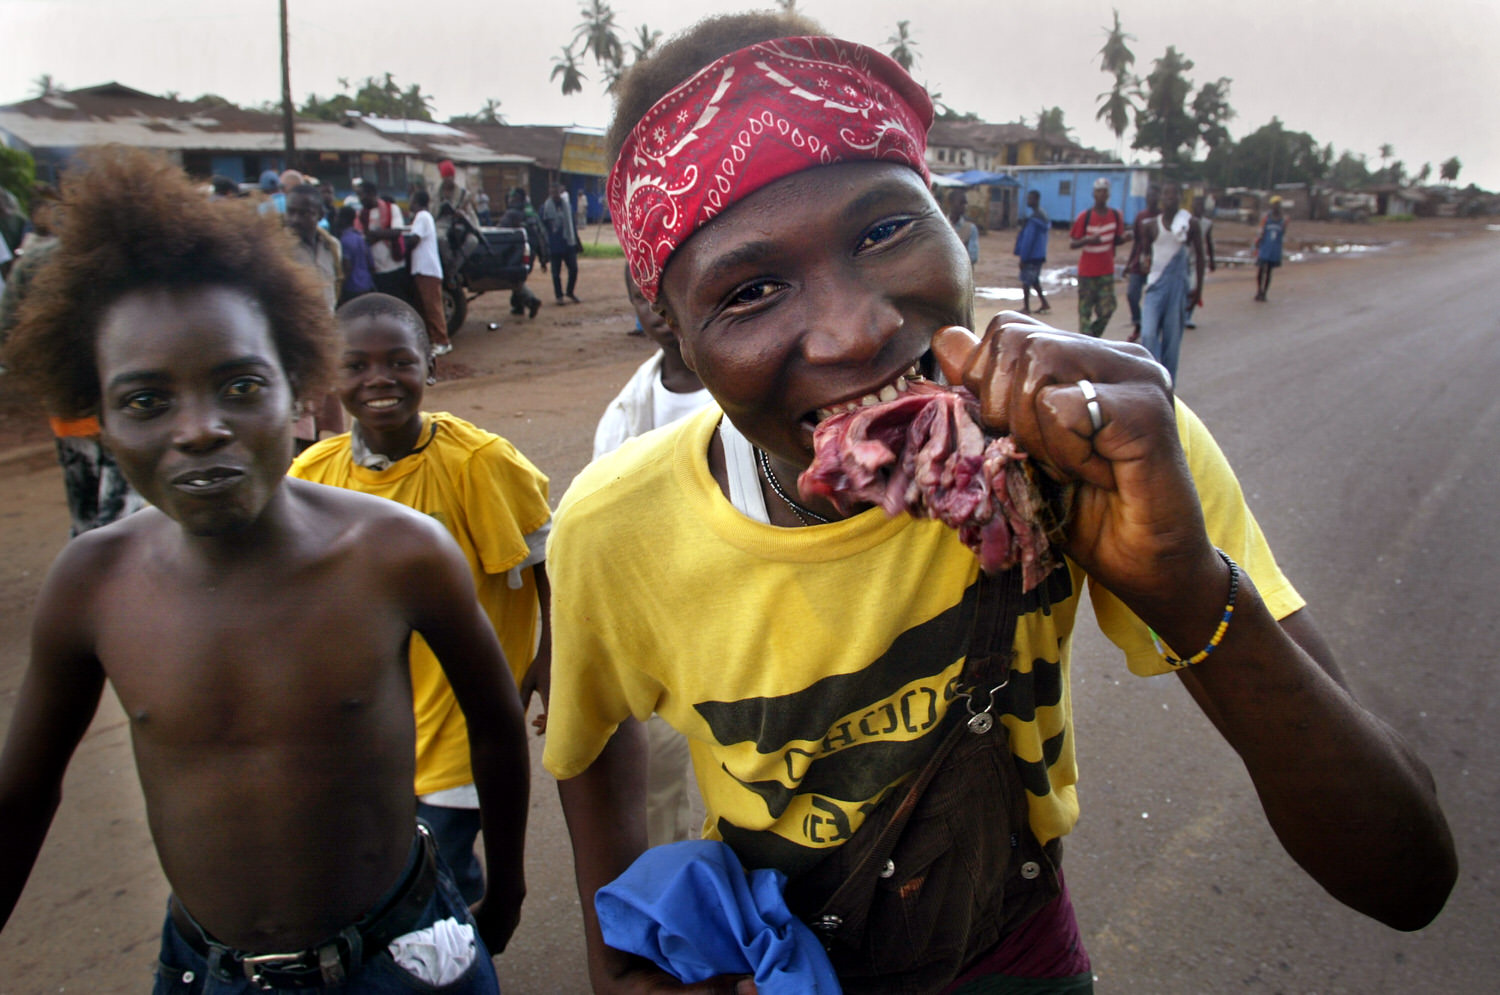
\includegraphics[width = 0.7\textwidth]{img/liberia_curtis}

{\footnotesize Liberian Civil War (Ben Curtis)}\\\vspace{10pt}

\begin{itemize}
  \item End of the Cold War and the big ideologies
  \item \BGyellow{The New Wars}: resource-rich countries, warlords, brutality, no ideological motivations...
\end{itemize}

\end{frame}
% ----------------------------------------------------

% ----------------------------------------------------
\begin{frame}
\frametitle{Examples}
\centering

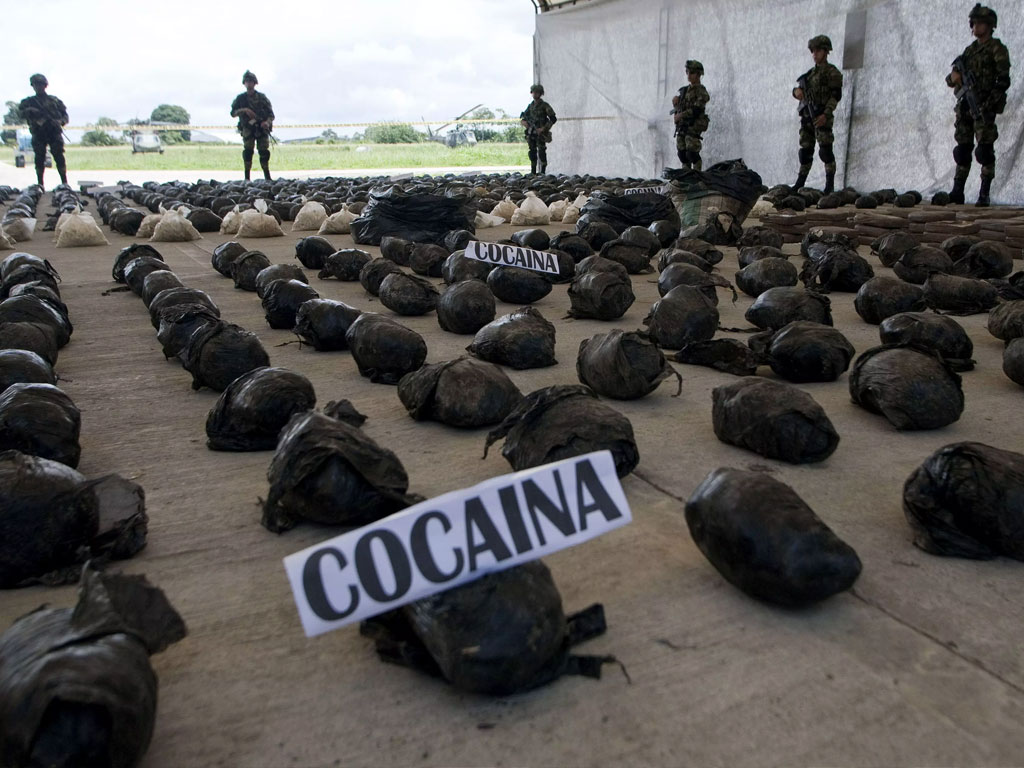
\includegraphics[width = 0.8\textwidth]{img/farc}

FARC and cocaine in Colombia

\end{frame}
% ----------------------------------------------------

% ----------------------------------------------------
\begin{frame}
\frametitle{Examples}
\centering

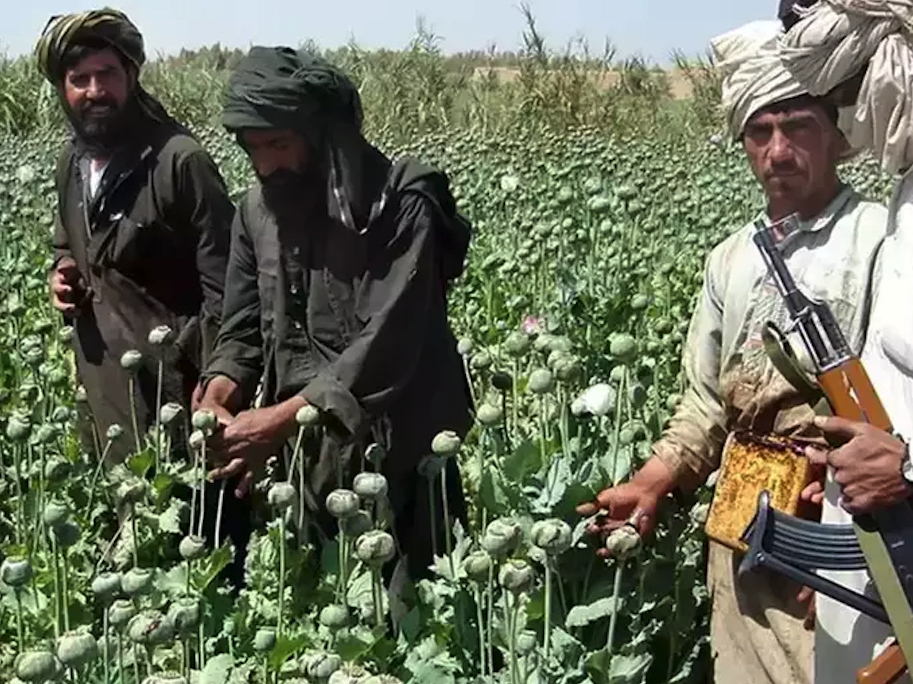
\includegraphics[width = 0.8\textwidth]{img/taliban}

Taliban and opium in Afghanistan

\end{frame}
% ----------------------------------------------------

% ----------------------------------------------------
\begin{frame}
\frametitle{Examples?}
\centering

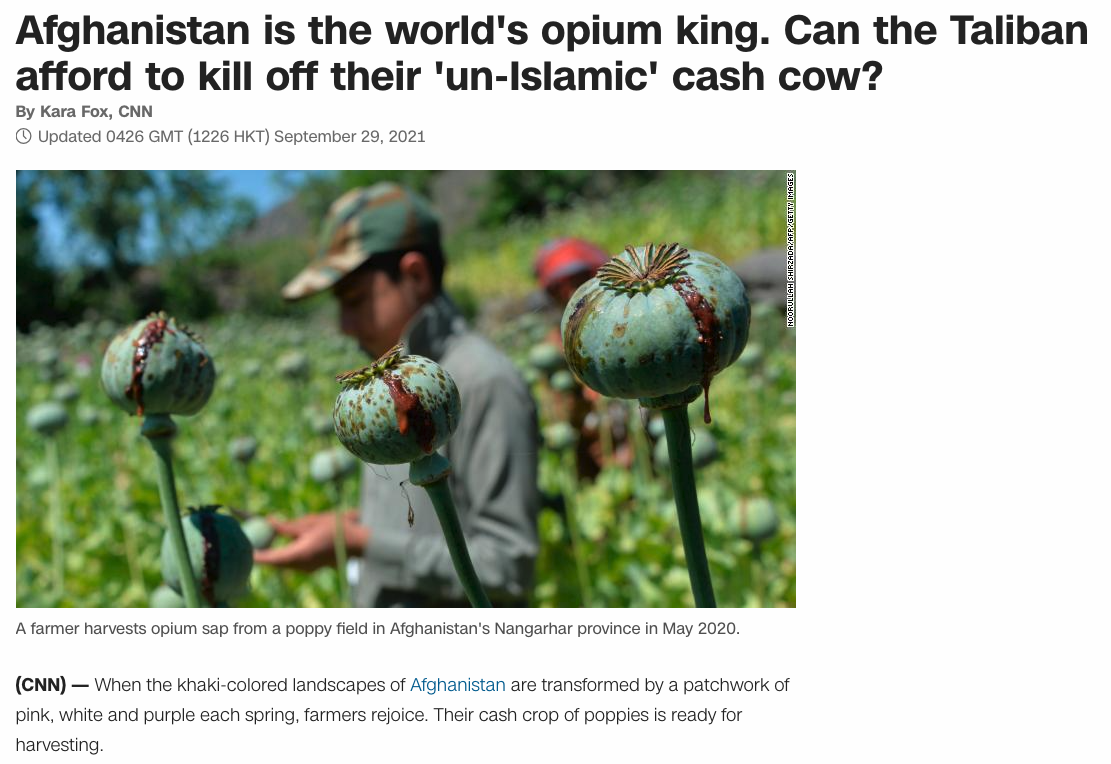
\includegraphics[width = 0.8\textwidth]{img/taliban_cnn}

\begin{itemize}
  \item By the way, how could we explain this?
  \begin{itemize}
    \item (i.e. Taliban trying to erradicate opium trade after getting power)
  \end{itemize}
\end{itemize}

\end{frame}
% ----------------------------------------------------

% ----------------------------------------------------
\begin{frame}
\frametitle{Implications}
\centering

\begin{minipage}{0.58\textwidth}\centering
\begin{itemize}
  \item Greed perspective is actually quite common {\small (not only for civil wars)}
  \item Not only about an academic debate on the causes, but with \textbf{major implications for conflict resolution}
  \begin{itemize}
    \item<2-> Which ones?
  \end{itemize}
  \item<3-> Related: Causes of onset $\neq$ organizational behavior
  \begin{itemize}
    \item Onset vs individual recruitment
    \item Taliban and oppium example
  \end{itemize}
\end{itemize}
\end{minipage}\hfill
\begin{minipage}{0.40\textwidth}\centering
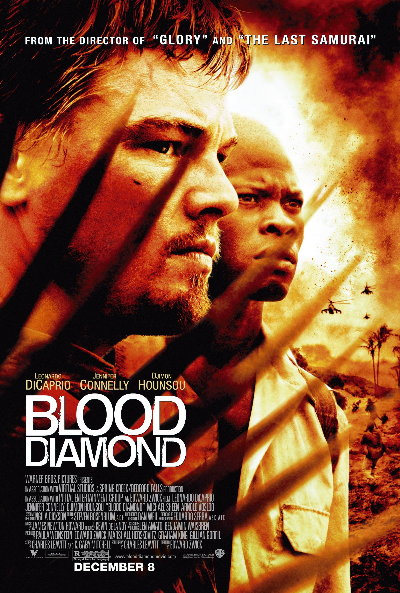
\includegraphics[width = 0.9\textwidth]{img/Blooddiamondposter}
\end{minipage}

\end{frame}
% ----------------------------------------------------

% ----------------------------------------------------
\begin{frame}
\frametitle{Refining \textit{greed} model: opportunity}
\centering

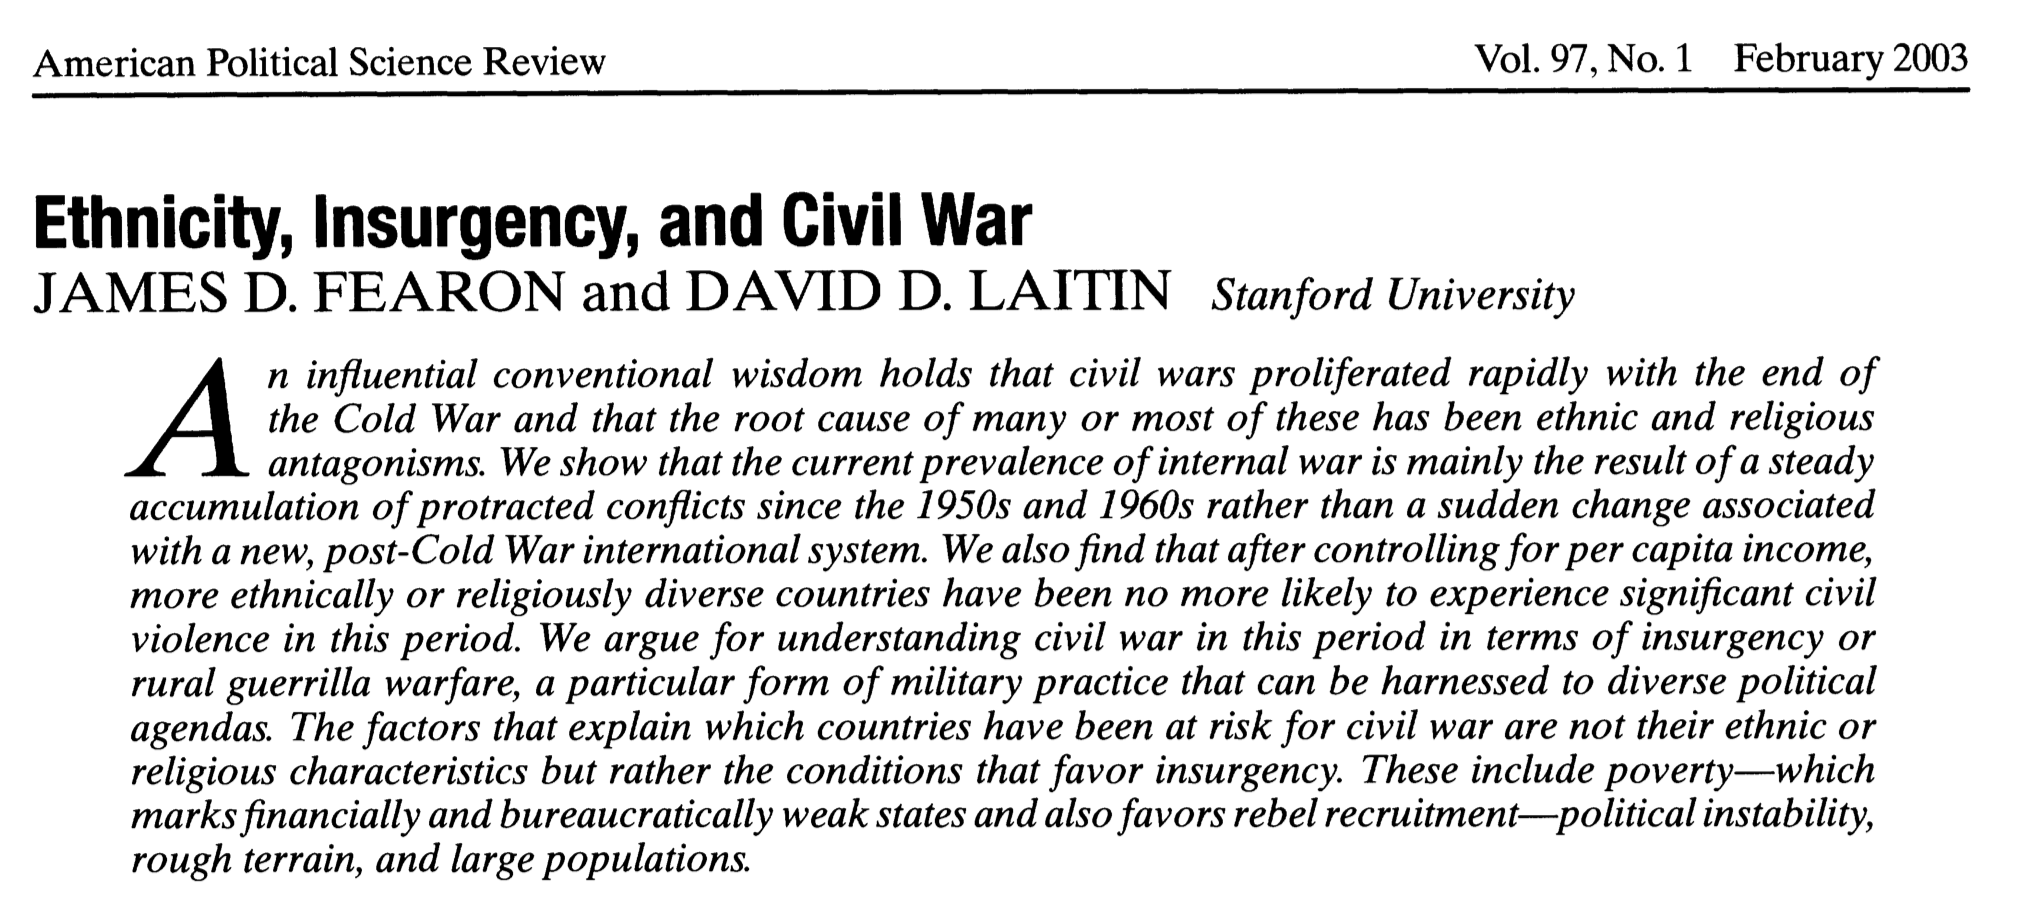
\includegraphics[width = \textwidth]{img/fearon_laitin}

\begin{itemize}
  % \item Fearon \& Laitin (2003) Ethnicity, Insurgency, and Civil War (\textit{American Political Science Review})
  \item Stressing \BGyellow{\textit{opportunity}} instead of greed
  \item Most influential explanation on civil war
  \begin{itemize}
    \item[] (most cited article in the main PolSci journal)
  \end{itemize}
\end{itemize}

\end{frame}
% ----------------------------------------------------

% ----------------------------------------------------
\begin{frame}
\frametitle{Fearon \& Laitin's model of insurgency}
\centering

\begin{itemize}
  \item It's not about greedy rebels calculating how to get rich
  \item Focus on the `\textbf{technology of insurgency}': factors that improve the capacity of rebels to launch an armed conflict using ``small, lighly armed bands practicing guerrilla warfare from rural base areas''
  \item<2-> Implication: \BGyellow{civil war erupts when the state is weak} (\& up for grabs by political opponents)
\end{itemize}

\end{frame}
% ----------------------------------------------------

% ----------------------------------------------------
\begin{frame}
\frametitle{Fearon \& Laitin's model of insurgency}
\centering

\begin{itemize}
  \item[] What makes these rural insurgencies more likely?
  \item \BGyellow<2>{Poverty}
  \begin{itemize}
    \item no capacity to police \& easier for the rebels to recruit
  \end{itemize}
  \item \BGyellow<3>{Rough terrain}
  \begin{itemize}
    \item easier for the rebels to organize, hide from the state
  \end{itemize}
  \item \BGyellow<4>{Political instability}
  \begin{itemize}
    \item disorganized center of power, less capacity to control
  \end{itemize}
  \item \BGyellow<5>{Large populations}
  \begin{itemize}
    \item again, more difficult to control and easier rebel recruitment
  \end{itemize}
  \item<6-> F\&L argued \textbf{ethnic and religious divisions had no effect}
\end{itemize}

\end{frame}
% ----------------------------------------------------

% ----------------------------------------------------
\begin{frame}
\frametitle{Fearon \& Laitin's diagnoses}
\centering

\begin{itemize}
  \item So why did we have so much war in the 1960s and 1990s?
\end{itemize}

\end{frame}
% ----------------------------------------------------

% ----------------------------------------------------
\begin{frame}
\frametitle{Fearon \& Laitin's diagnoses}
\centering

\begin{itemize}
  \item Focus on the `\BGyellow{\textbf{resource curse}}': countries that depend on natural resources are more likely to suffer insurgencies and conflict
  \item<2-> Collier \& Hoeffler's \textbf{greed model}: they are easy to loot
  \item<2-> Fearon \& Laitin's \textbf{opportunity model}: resource-rich countries don't need to develop tax extraction and public services, leading to bad governance and weak institutions
  \item<3-> Particularly much worse in countries with rough terrain and peripherical regions
  \begin{itemize}
    \item Remember Tilly's model of state creation? if you have oil or diamonds, no need to develop state structures for taxation
  \end{itemize}
\end{itemize}

\end{frame}
% ----------------------------------------------------

% ----------------------------------------------------
\begin{frame}
\frametitle{Fearon \& Laitin's diagnoses}
\centering

\begin{minipage}{0.58\textwidth}\centering
\begin{itemize}
  \item That should be the \textbf{main reason} behind the post-1960 increase in civil war
  \item \textbf{Not} because of grievances related to the decolonization process, but because these states were `half-baked'
  \item (Same argument applies to Latin America, according to them)
\end{itemize}
\end{minipage}\hfill
\begin{minipage}{0.4\textwidth}\centering
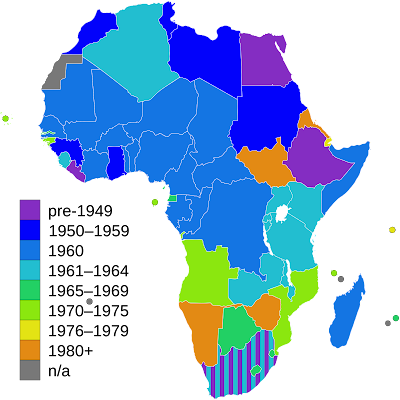
\includegraphics[width = \textwidth]{img/africa_decolonization}\\
Decolonization in Africa
\end{minipage}

\end{frame}
% ----------------------------------------------------

% ----------------------------------------------------
\begin{frame}
\frametitle{Fearon \& Laitin's diagnoses}
\centering

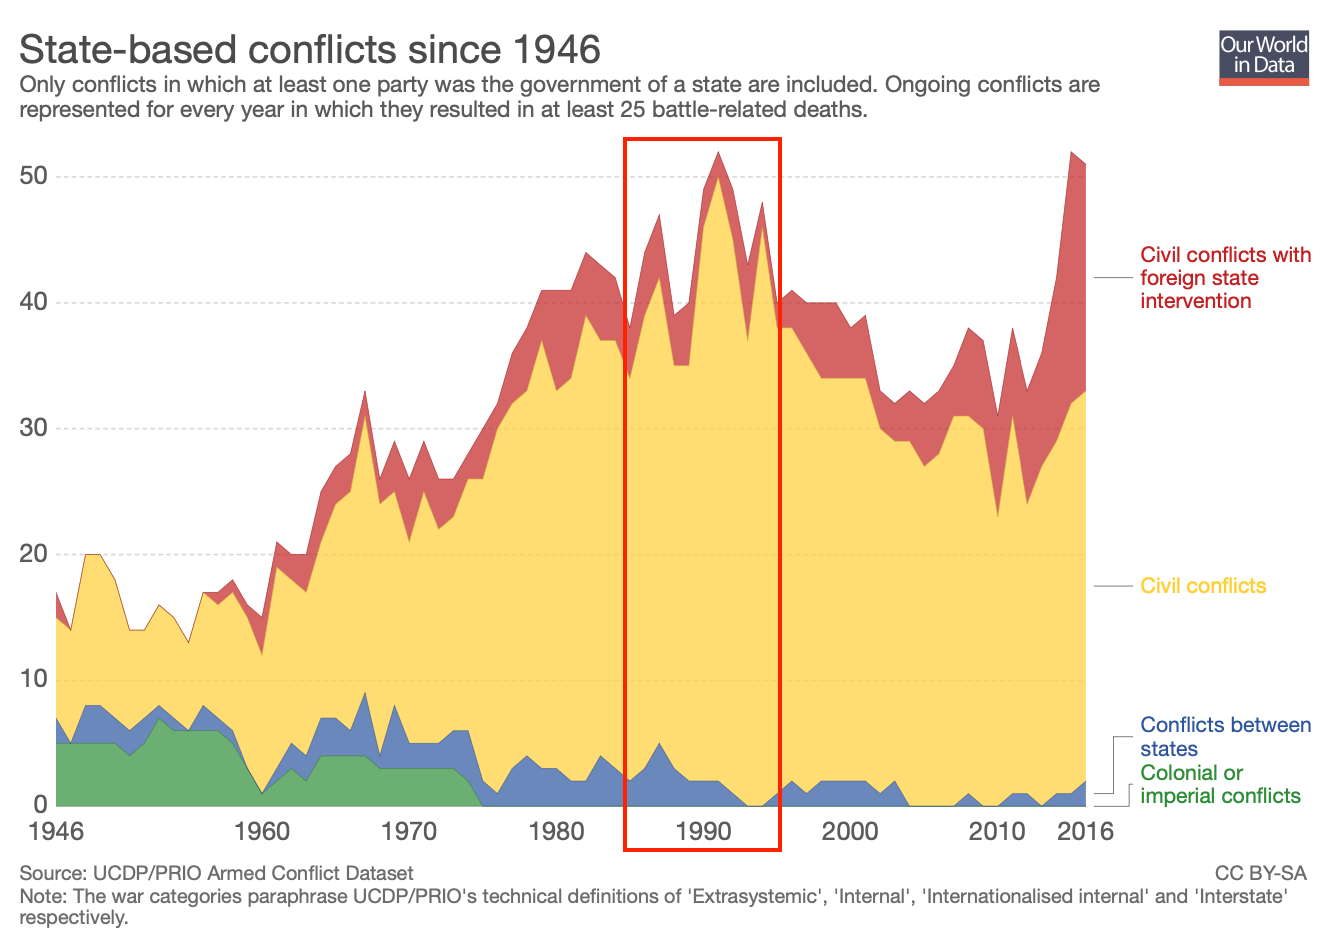
\includegraphics[width = 0.75\textwidth]{img/conflicts_over_time90}

\begin{itemize}
  \item What about the 1990s?
  \begin{itemize}
    \item civil war incidence \textit{appeared} to rise after the end of the Cold War
  \end{itemize}
\end{itemize}

\end{frame}
% ----------------------------------------------------

% ----------------------------------------------------
\begin{frame}
\frametitle{Fearon \& Laitin's diagnoses}
\centering

\begin{itemize}
  \item Previous explanations on the role of the international system or the rise of multi-ethnic countries
  \item<2-> Fearon \& Laitin: it's not new wars but the \textbf{consequence of many} \BGyellow{\textbf{protracted conflicts}} \textbf{that have not still ended}, brought about by the new weak states created in the decolonization waves of the 1950s and 1970s
  \item<3-> Implication? We should focus on the technology of insurgency, the \textit{domestic} conditions that favor rebellion, but not on the international level or on cultural, ethnic, or religious differences
\end{itemize}

\end{frame}
% ----------------------------------------------------

% ----------------------------------------------------
\begin{frame}
\frametitle{Extensions}
\centering

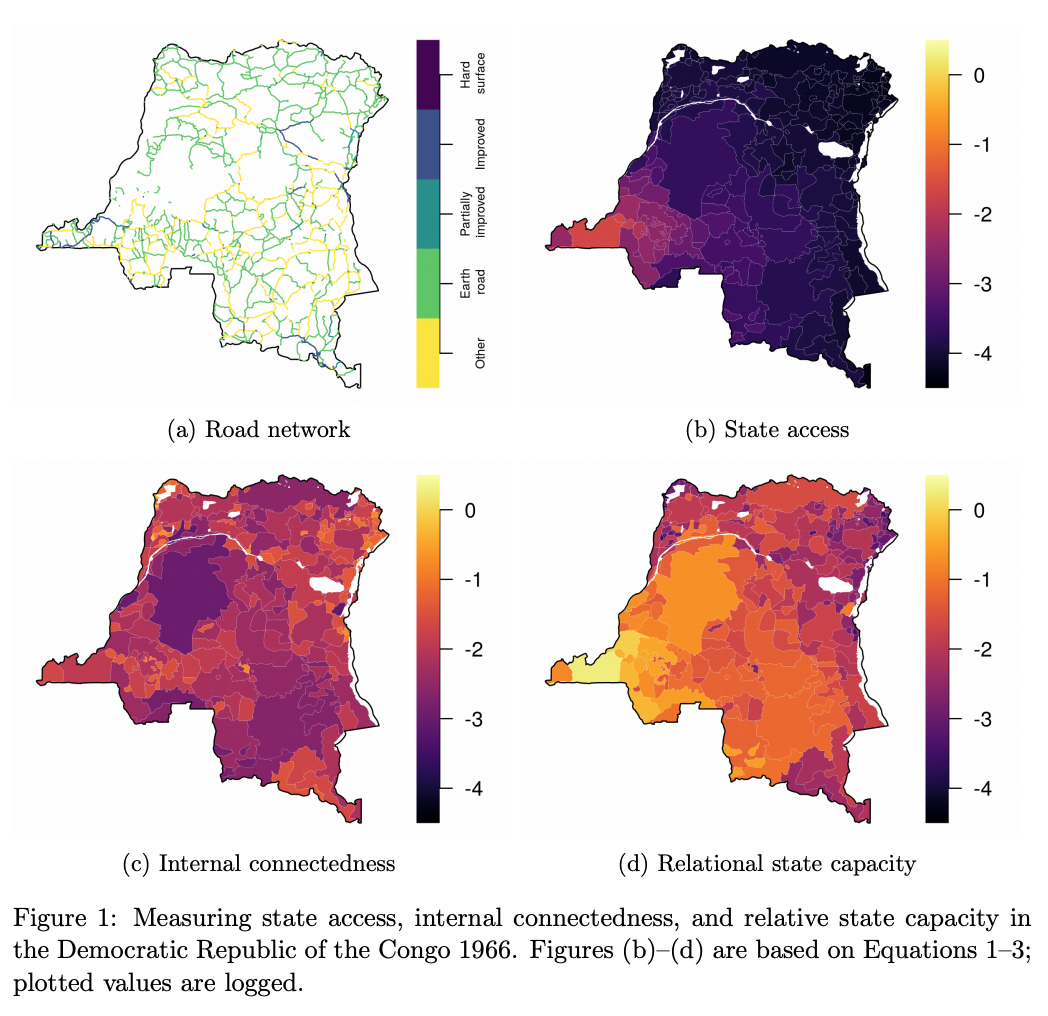
\includegraphics[width = 0.75\textwidth]{img/muller-crepon}

\end{frame}
% ----------------------------------------------------

% ----------------------------------------------------
\begin{frame}
\frametitle{Extensions}
\centering

\begin{itemize}
  \item Concept of \textbf{relational state capacity}
  \item Empirical methods
  \item Reference:
  \begin{itemize}
    \item {\small Carl Müller-Crepon, Philipp Hunziker, and Lars-Erik Cederman (2021) Roads to Rule, Roads to Rebel: Relational State Capacity and Conflict in Africa. \textit{Journal of Conflict Resolution} 65(2--3): 563--590.}
  \end{itemize}
\end{itemize}

\end{frame}
% ----------------------------------------------------

% ----------------------------------------------------
\begin{frame}
\frametitle{Next week}
\centering

\begin{itemize}
  \item About how we learned the way grievances and inequality also matter
  \item And on other aspects of civil wars: duration, international factors...
\end{itemize}

\end{frame}
% ----------------------------------------------------

% ----------------------------------------------------
\begin{frame}
\frametitle{Next seminar}
\centering

\begin{minipage}{0.55\textwidth}\centering
\begin{itemize}
  \item Robert D Kaplan, `The coming anarchy' (\textit{The Atlantic,} 1994)
  \item Pessimist view on Post-Cold War international security
\end{itemize}
\end{minipage}\hfill
\begin{minipage}{0.44\textwidth}\centering
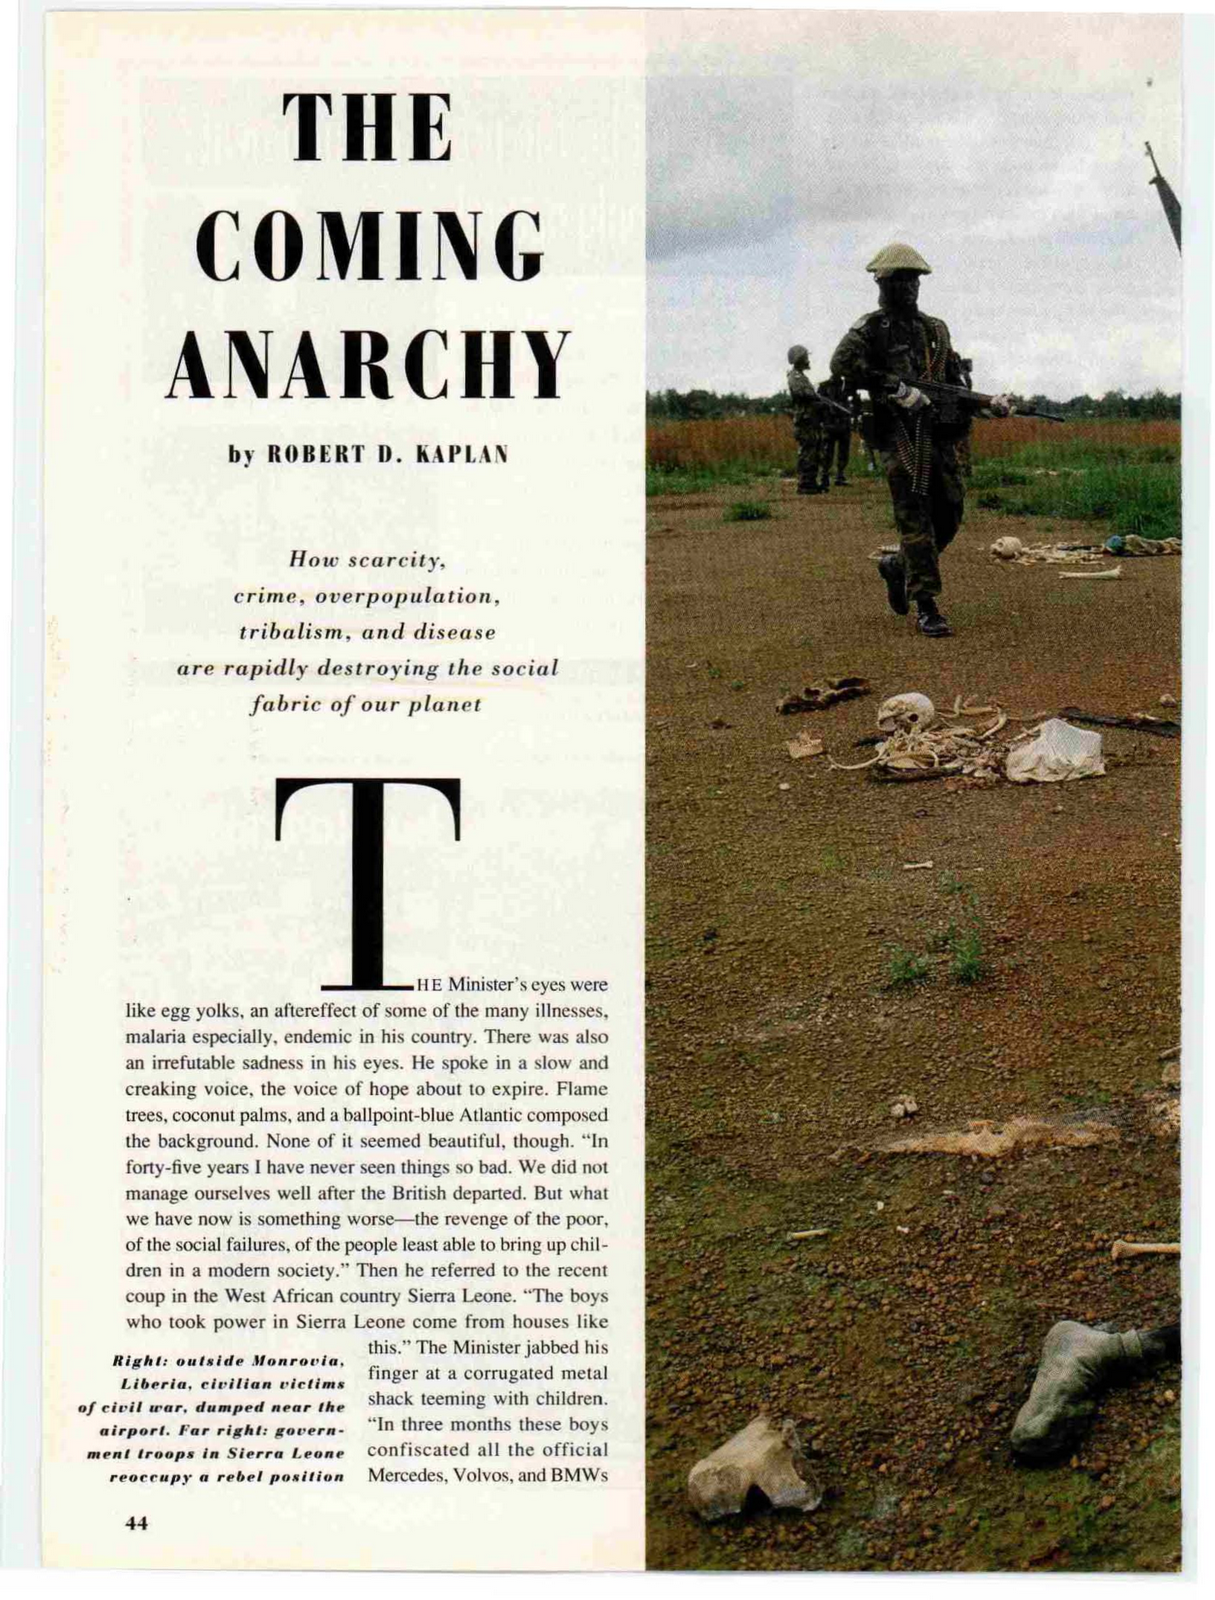
\includegraphics[width = \textwidth]{img/ComingAnarchy}
\end{minipage}

\end{frame}
% ----------------------------------------------------


\end{document}
